\documentclass[12pt]{article}  % 官方要求字号不小于 12 号,此处选择 12 号字体
% \linespread{1.1}
% \bibliographystyle{plain}
% 本模板不需要填写年份,以当前电脑时间自动生成
% 请在以下的方括号中填写队伍控制号
\usepackage[]{easymcm}  % 载入 EasyMCM 模板文件
\usepackage{palatino}  
\usepackage{pdfpages}
\usepackage{longtable}
\usepackage{tabu}
\usepackage{threeparttable}
\usepackage{listings}
\usepackage{paralist}
\usepackage{setspace}
\usepackage{CJKutf8}
\usepackage{textcomp} % 必须加上,否则报错
\usepackage{ctex}
\usepackage{listings} %插入代码
\usepackage{xcolor} %代码高亮
\usepackage{amsmath}
\usepackage{algorithmic}
\usepackage{algorithm}

\makeatletter
\newenvironment{breakablealgorithm}
{% \begin{breakablealgorithm}
		\begin{center}
			\refstepcounter{algorithm}% New algorithm
			\hrule height.8pt depth0pt \kern2pt% \@fs@pre for \@fs@ruled
			\renewcommand{\caption}[2][\relax]{% Make a new \caption
				{\raggedright\textbf{\ALG@name~\thealgorithm} ##2\par}%
				\ifx\relax##1\relax % #1 is \relax
				\addcontentsline{loa}{algorithm}{\protect\numberline{\thealgorithm}##2}%
				\else % #1 is not \relax
				\addcontentsline{loa}{algorithm}{\protect\numberline{\thealgorithm}##1}%
				\fi
				\kern2pt\hrule\kern2pt
			}
		}{% \end{breakablealgorithm}
		\kern2pt\hrule\relax% \@fs@post for \@fs@ruled
	\end{center}
}
\makeatother

\lstset{numbers=left, %设置行号位置
	numberstyle=\tiny, %设置行号大小
	breaklines=true
	keywordstyle=\color{blue}, %设置关键字颜色
	commentstyle=\color[cmyk]{1,0,1,0}, %设置注释颜色
	frame=single, %设置边框格式
	escapeinside=``, %逃逸字符(1左面的键),用于显示中文
	extendedchars=false, %解决代码跨页时,章节标题,页眉等汉字不显示的问题
	xleftmargin=2em,xrightmargin=2em, aboveskip=1em, %设置边距
	tabsize=4, %设置tab空格数
	showspaces=false %不显示空格
}

\let\itemize\compactitem
\let\enditemize\endcompactitem
\newcommand{\upcite}[1]{\textsuperscript{\textsuperscript{\cite{#1}}}}

\title{摘要} 

% 文档开始
\begin{document}
\begin{abstract}
	\vspace{15pt}
	本项目围绕机器学习分类算法展开,以支持向量机(support vector machine, SVM)为主要研究对象,探究其分类性能、模型改进与优化算法。SVM和Logistic回归模型都可以用于解决二分类问题,但模型设计的思路不同,因此希望能够比较两者在分类性能上的差异。项目过程中代码完全基于R语言实现,主要以二维样本数据为研究对象,生成模拟数据并基于经典硬间隔SVM模型和Logistic回归模型分别进行建模与训练,在测试集上对模型进行验证,最终比较两者的分类效果差异。实验结果表明,当样本数据本身区分度不明显时,两种分类模型效果均较差,但Logistic模型明显优于经典硬间隔SVM;当样本数据本身具有明显的差异性时,两种分类模型效果均较好,SVM略优于Logistic。此外,还对改进后的SVM模型(核函数由线性函数更换为高斯核函数)进行性能测试,发现其在区分度不明显的数据集上显著优于经典硬间隔SVM,说明其显著提升了其在非线性可分数据上的分类效果;但在区分度较明显的数据集上分类效果反而略逊于经典SVM模型。最后,对两篇有关SVM改进模型的文献进行了阅读与调研,总结了软间隔SVM模型在正则项和损失项拓展方面的研究进展,并介绍了柔性套索惩罚和快速截断Huber损失等改进方法。
	\vspace{5pt}
	\noindent
	
	\textbf{关键词}: 机器学习分类算法、二分类、支持向量机(SVM)、Logistic回归、硬间隔、软间隔、高斯核函数、改进的SVM模型、柔性套索惩罚、快速截断Huber损失、R语言
\end{abstract}

\maketitle  

\tableofcontents

\section{项目概述}

\subsection{问题背景}
人工智能的概念是在1956年首次被提出,其目标旨在希望通过计算机模拟人的思维能力或智能行为,从而让计算机能够像人类一样进行思考。目前,人工智能已经在机器翻译、智能控制、图像识别、语音识别、游戏博弈等领域得到广泛的应用。

机器学习作为人工智能的一个发展方向,起源于20世纪50年代的感知机数学模型,其目标是使得机器能够像人类一样具有学习能力。机器学习的基本过程主要是基于样本数据(客体)去训练/学习某个模型或决策函数(主体)。一般而言,正则化框架下的机器学习过程主要由\textbf{学习机、损失项和正则项(惩罚项)}三个部分构成,最终通过学习得到模型。

\begin{figure}[H]
	\centering
	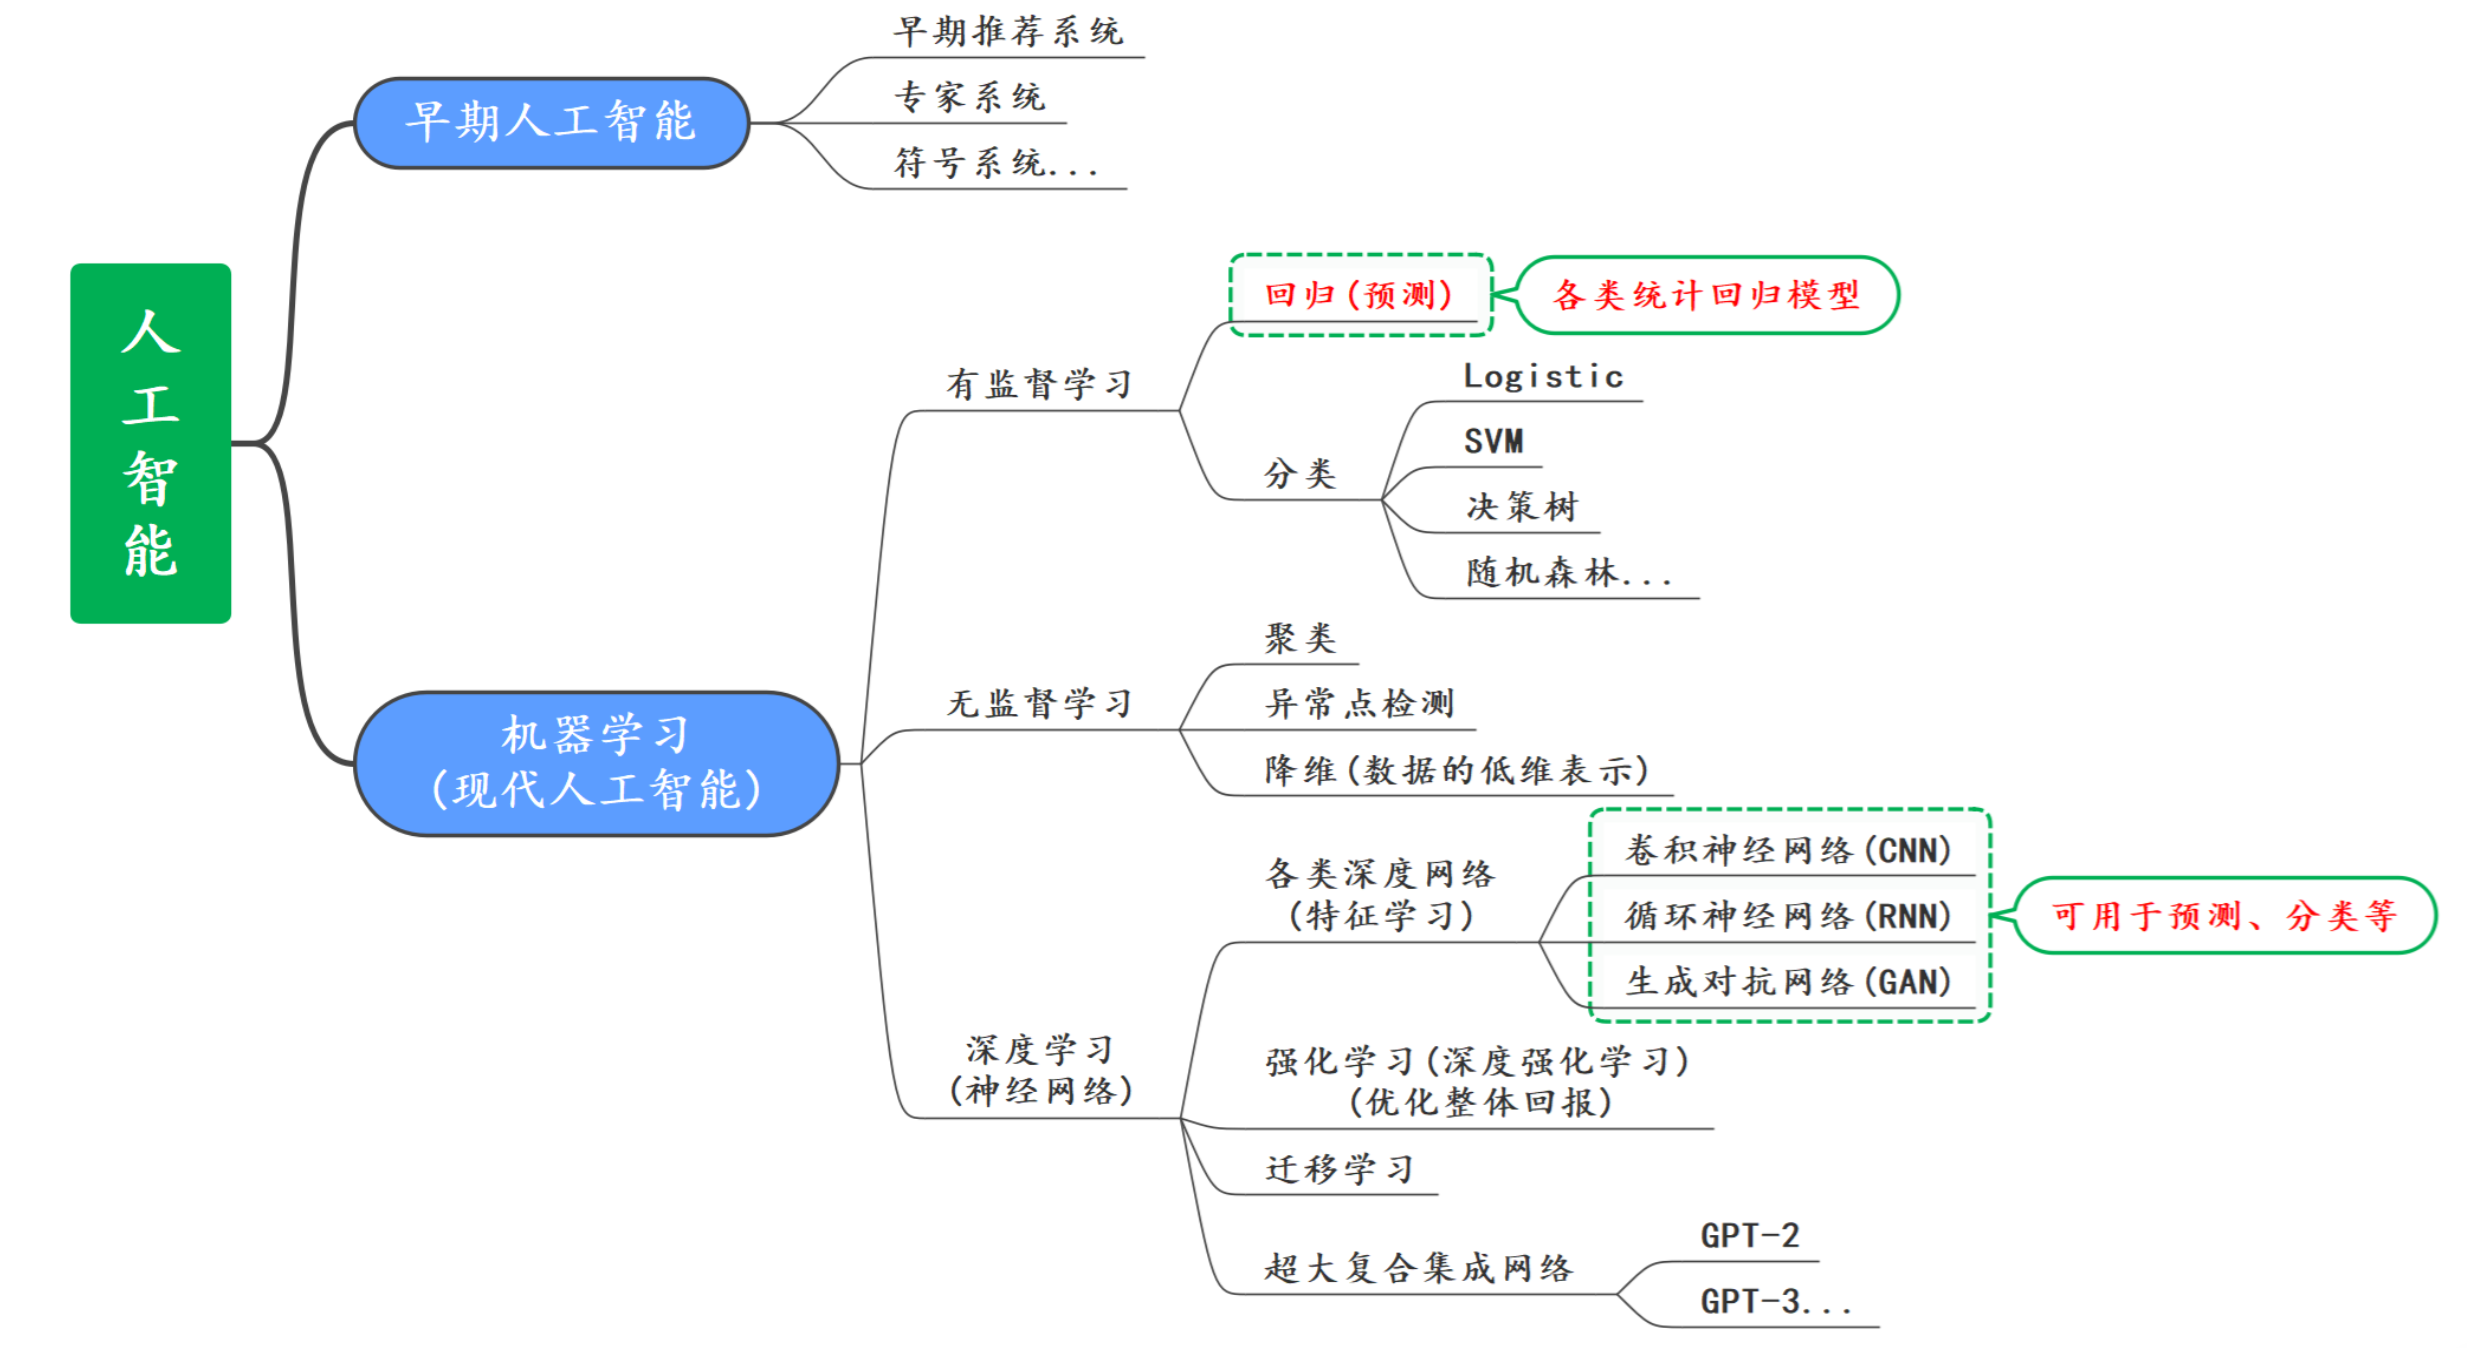
\includegraphics[width=0.8\textwidth]{1.png}
\end{figure}

支持向量机(support vector machine,SVM)最早由Cortes和Vapnik二人于1995年为解决二分类问题而提出\upcite{1}。 作为经典的机器学习模型之一,SVM有坚实的统计理论基础,算法实现容易,且决策函数具有很强的几何含义。由于其在模式识别等数据分析问题中的优越表现,SVM如今已成为最经典的判别分析方法之一。与SVM相类似,广义线性回归统计模型中的Logistic回归模型同样也可用于解决二分类问题。本质上来说,两种方法都注重研究一组协变量$X_1,⋯,X_p$是如何影响二元的响应变量$Y$的,在用途上具有极大的相似性,因而希望研究并比较两者分类效果的差异性。

除此之外,SVM作为一种经典且基础的机器学习算法,在漫长的发展历程中也经历了多次迭代,有多种多样的改进版本。最基本的版本为硬间隔SVM,但由于实际的样本数据很可能不满足线性可分的理想情况,又发展出了采用不同求解算法的软间隔SVM模型以及基于核函数升维思想实现的非线性SVM,基于软间隔SVM模型又集中在模型损失项与正则项两个方面进行了理论上的拓展。这样的发展是永无止境的,在此希望对过去的部分研究改进成果进行理论总结与代码实现,以更好地了解SVM模型的发展现状。

\subsection{项目任务}	

在本次项目中,需要随机生成模拟数据,并在该样本数据基础上分别利用经典SVM模型与Logistic模型进行统计建模,同时对比两者的分类效果;此外还需要总结并实现部分改进版本的SVM算法,分析其预测效果。具体而言可细分为如下任务:
\begin{itemize}
	\setlength{\parsep}{0ex} %段落间距
	\setlength{\topsep}{2ex} %列表到上下文的垂直距离
	\setlength{\itemsep}{1ex} %条目间距
	\item \textbf{任务 1}:随机生成200条模拟数据并将其分为训练数据集与测试数据集,利用训练数据集分别基于经典硬间隔SVM模型与Logistic广义线性回归模型建立统计模型,实现样本数据的分类且在测试数据集上进行验证,比较两者的分类效果差异。		
	\item \textbf{任务 2}:代码实现某一种改进版本的SVM模型,简单测试其性能并将其分类结果与经典版本进行对比。
	\item \textbf{任务 3}:查阅SVM模型改进相关的文献,基于正则化框架对于文献中涉及的模型(学习机、损失项、正则项)、创新点与求解算法进行重述与总结。
\end{itemize}

\section{项目过程}
本项目代码部分完全基于R语言实现,主要涉及样本模拟数据的生成,以及SVM(经典与改进版本)与Logistic回归模型的建立、训练与测试。
\subsection{模拟数据生成}
本项目中涉及到的样本数据完全由模拟方法生成。具体而言,不论是SVM还是 Logistic回归模型,其目的都是为了研究一系列协变量对于一个二元的响应变量的影响。为方便起见,选择采用协变量的维度为\textbf{二维},即二元响应变量$Y$只由两个变量$X_1,X_2$决定。在生成数据时,为了较好地区分出两类数据,分别在正态总体下以均值为0和均值为1生成两组模拟数据(同一条数据中的两个变量$X_1,X_2$来自同一均值的总体),并分别打上分类标签(即对应$Y$的取值为)0或1:

\begin{lstlisting}[language=R]
	set.seed(123) #设置随机种子,固定每次运行程序生成的随机数,使结果可重复
	n <- 200  # 每个类别的数据点数
	
	# 生成类别0的数据
	x1 <- matrix(rnorm(n * 2, mean = 0), ncol = 2)
	y1 <- rep(0, n)
	# 生成类别1的数据
	x2 <- matrix(rnorm(n * 2, mean = 1), ncol = 2)
	y2 <- rep(1, n)
	# 合并数据
	x <- rbind(x1, x2)
	y <- c(y1, y2)
\end{lstlisting} 

绘制样本点对应的散点图,初步观察其分类情况:
\begin{lstlisting}[language=R]
	# 加载 ggplot2 包
	library(ggplot2)
	
	# 创建数据框
	data <- data.frame(x1 = x[, 1], x2 = x[, 2], y = factor(y))
	
	# 设置点的大小和透明度
	p <- ggplot(data, aes(x = x1, y = x2, color = y)) +
	geom_point(size = 3, alpha = 0.7) +  # 调整点的大小和透明度
	scale_color_manual(values = c("blue", "red")) +
	labs(x = "x1", y = "x2", color = "Class") +
	theme_minimal()
	
	# 调整背景和边界线
	p + theme(panel.background = element_rect(fill = "white", color = "black"),
	panel.border = element_rect(color = "black", fill = NA),
	axis.line = element_line(color = "black"))
	
	ggsave("2.png", plot = p, width = 6, height = 6, units = "in", dpi = 300)
\end{lstlisting}

\begin{figure}[H]
	\centering
	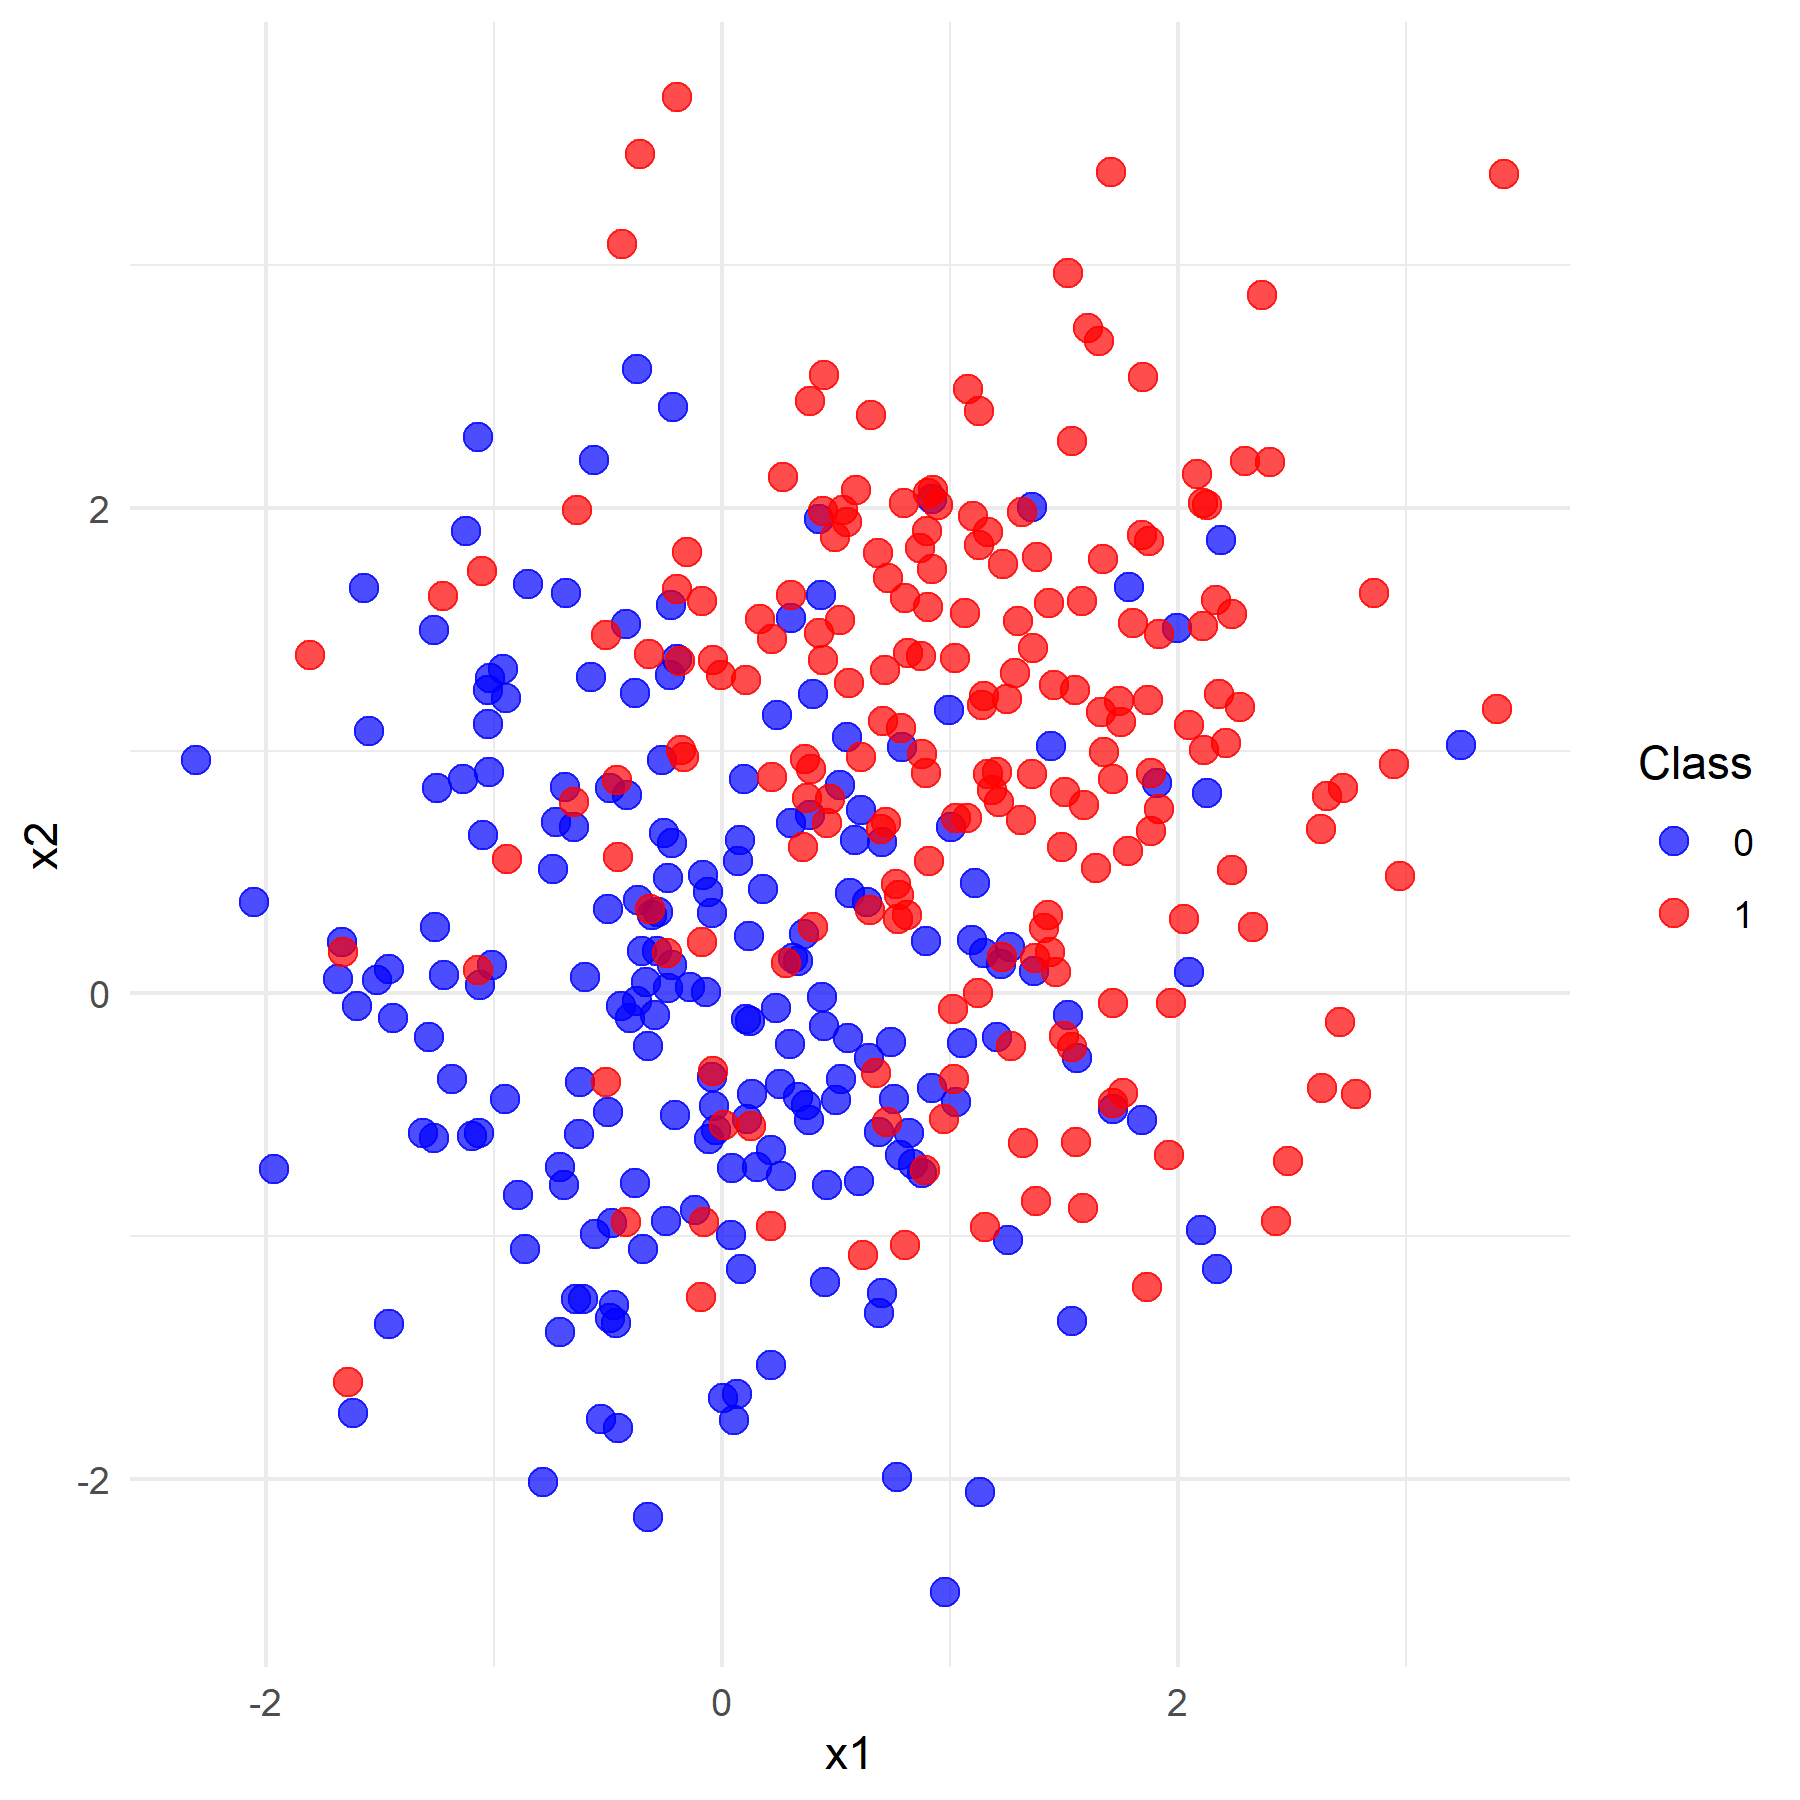
\includegraphics[width=0.4\textwidth]{2.png}
	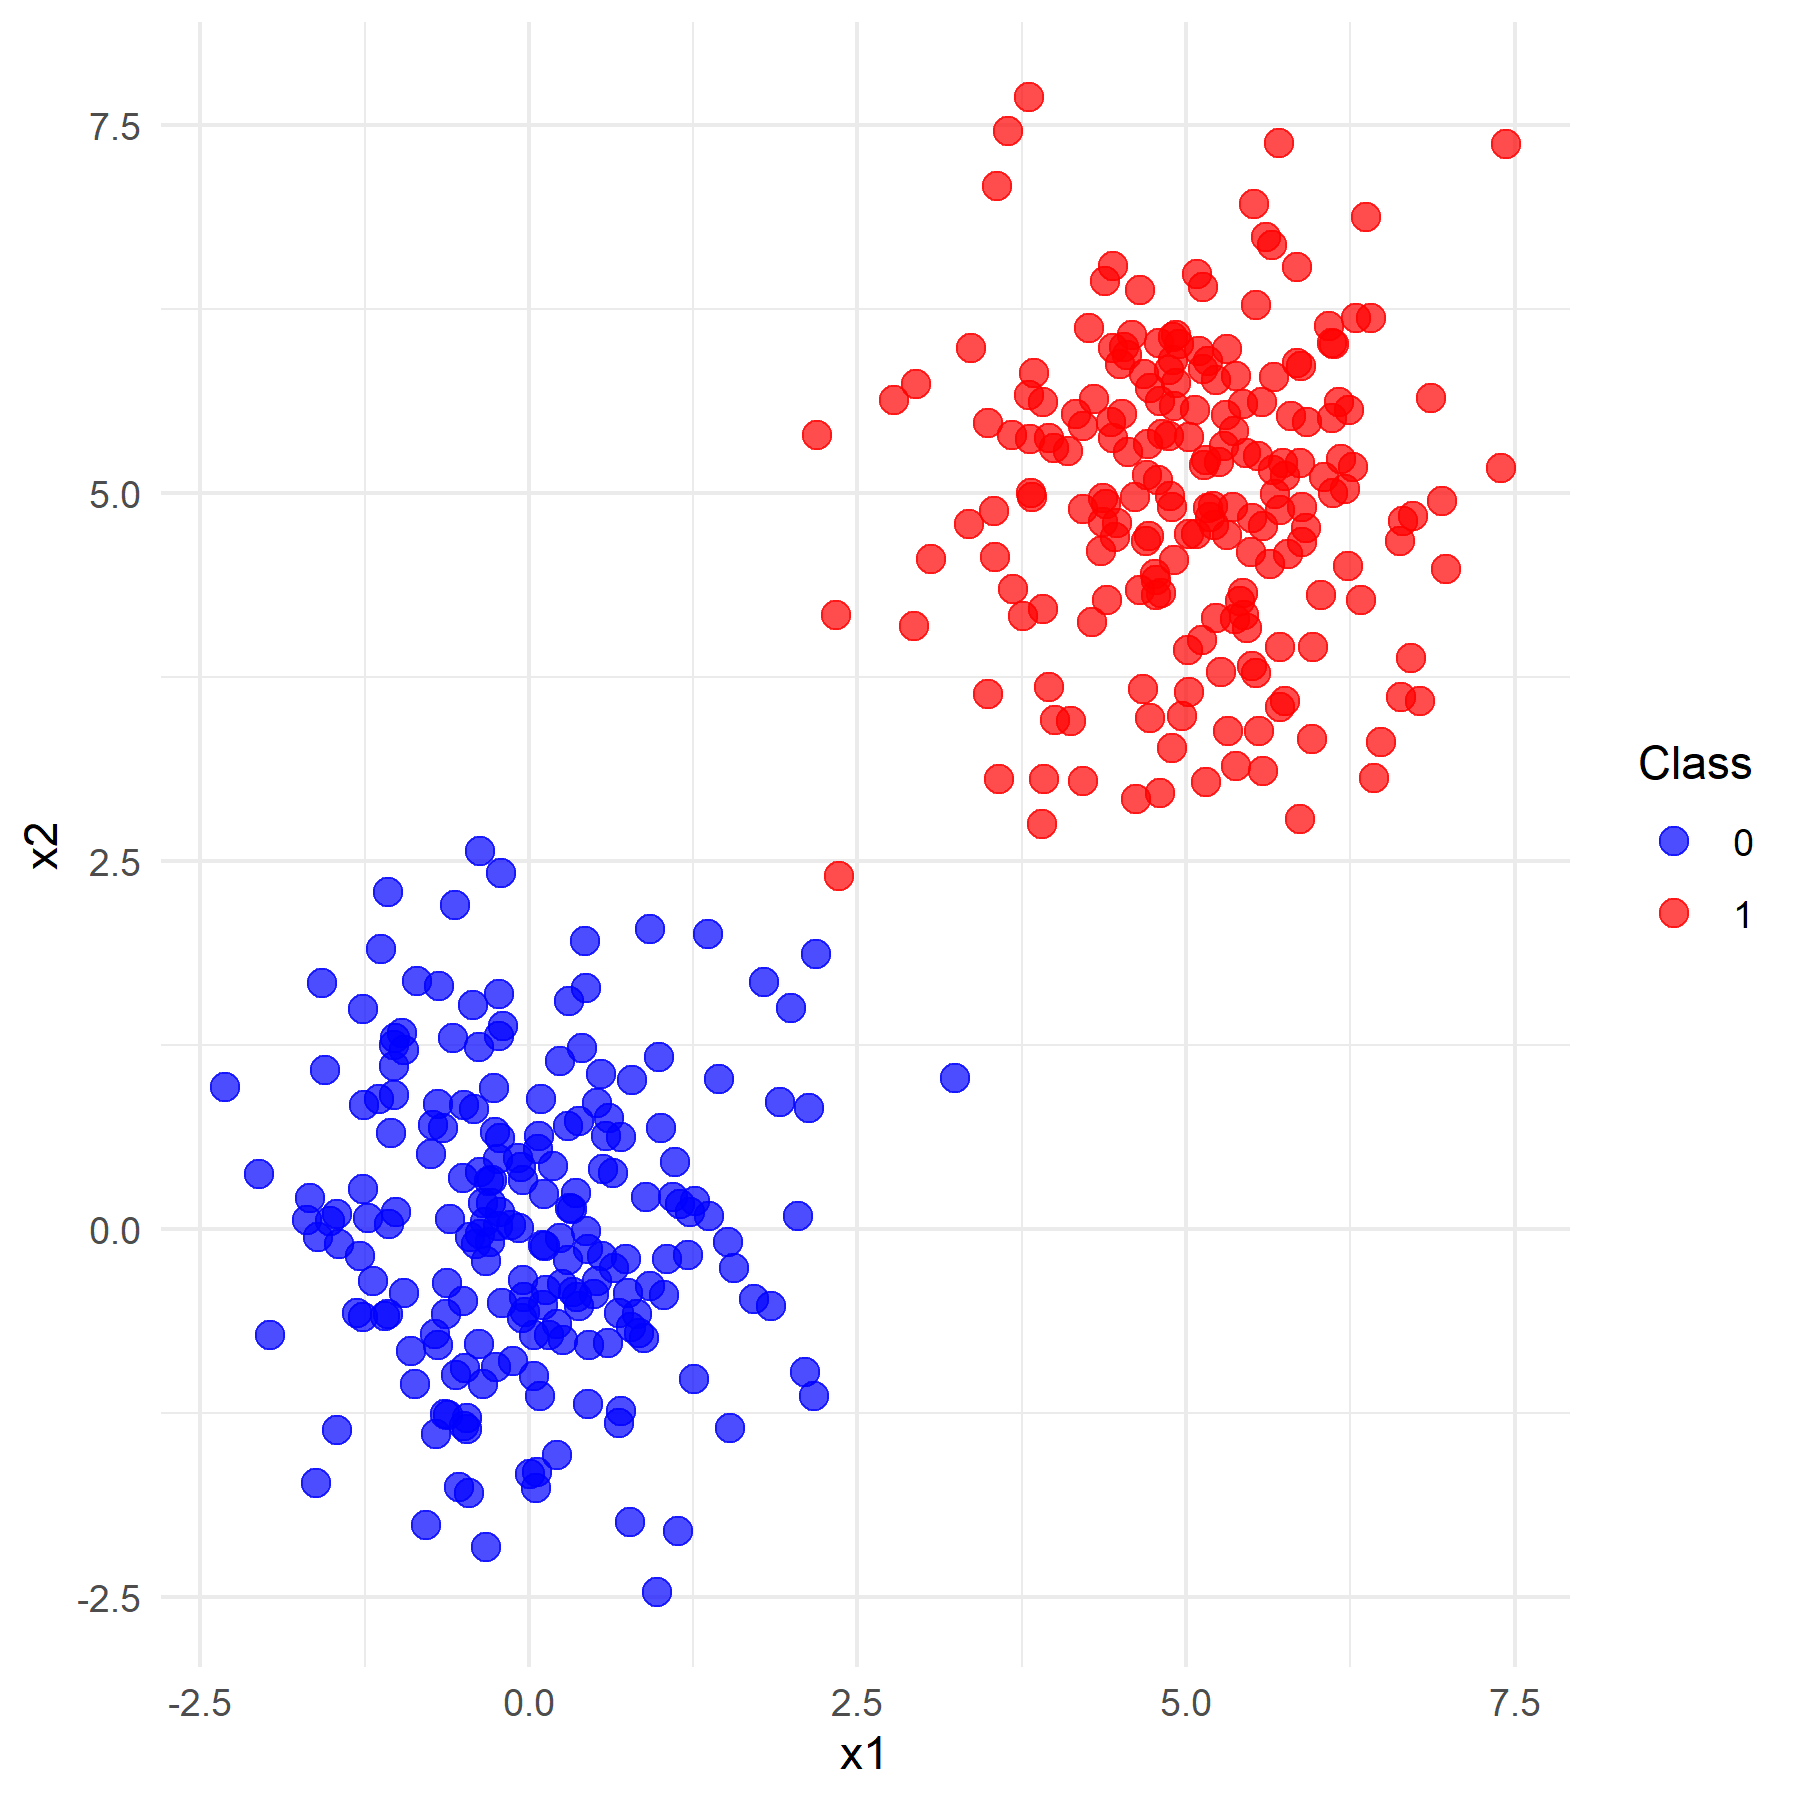
\includegraphics[width=0.4\textwidth]{3.png}
\end{figure}

观察上左图可知,由于基于正态总体生成模拟数据时仅制定了均值而未指定方差(默认为1),导致令均值为0和1的情况下两类数据没有办法明显的区分开来,这样的分类效果显然是不好的。经过调试,当设置两类数据均值分别为0和5时,数据点呈现良好的区分性(如上右图所示)。

为便于后续的模型训练,还需要将样本模拟数据分成训练集与测试集两部分,根据经验,较为合适的数据集数量比例为7:3,即样本数据中的$70\%$为训练集,另外$30\%$为测试集用于验证。

\begin{lstlisting}[language=R]
	# 将数据分为训练集和测试集
	train_index <- sample(1:(2 * n), 0.7 * 2 * n)
	x_train <- x[train_index, ]
	y_train <- y[train_index]
	x_test <- x[-train_index, ]
	y_test <- y[-train_index]
	
	# 合并 
	train_data <- cbind(x_train, y_train)
	test_data <- cbind(x_test, y_test)
\end{lstlisting}

在此对部分训练集数据进行罗列:

\begin{lstlisting}[language=R]
	#观察数据集
	head(train_data,10)
\end{lstlisting}

\begin{longtable}[]{@{}llllll@{}}
	\toprule\noalign{}
	 & x.1 & x.2 & y \\
	\midrule\noalign{}
	\endhead
	\bottomrule\noalign{}
	\endlastfoot
	
	1 & 5.8641525 & 2.78936689 & 1 \\
	2 & -1.9666172 & -0.72306597 & 0 \\
	3 & 0.8215811 & -0.57438869 & 0 \\
	4 & -1.2512714 & 0.84573154 & 0 \\
	5 & 1.3686023 & 0.09049665 & 0 \\
	6 & -0.2153805 & 2.41677335 & 0 \\
	7 & 6.0466288 & 5.10719041 & 1 \\
	8 & 1.0057385 & 0.68430943 & 0 \\
	9 & 4.6738561 & 3.67224452 & 1 \\
	10 & -0.4727914 & -1.28471572 & 0 \\
\end{longtable}

\subsection{基于经典硬间隔SVM模型的建模}

硬间隔支持向量机是一种基于\textbf{线性可分数据集}的分类模型。线性可分,意味着可用一条直线将两类数据分开。显然这样的直线有无穷多条,但对应直线的上下移动又因分类要求的限制而存在极限位置。因此,硬间隔支持向量机所要解决的\textbf{关键问题}就是,\textbf{如何从无穷多条直线(对应无穷多个分类器)中选择最优}?

实际上,具有“最大间隔”的分类器就是SVM要寻找的最优解,而最优解对应的两侧虚线(上下极限状态)所穿过的样本点,就是SVM中的支持样本点,称为\textbf{"支持向量"}。SVM中寻找最优分类器的问题,本质上是一个优化问题。对于一般的优化问题,往往有3个基本要素需要重点关注:

\begin{itemize}
	\setlength{\parsep}{0ex} %段落间距
	\setlength{\topsep}{2ex} %列表到上下文的垂直距离
	\setlength{\itemsep}{1ex} %条目间距
	\item \textbf{目标函数}:希望优化的目标指标;		
	\item \textbf{优化对象}:期望通过改变哪些因素(协变量)使目标函数达到最优;
	\item \textbf{约束条件}:优化对象一般需要满足一些特定的约束条件。
\end{itemize}

假定${{({x_i}^T,y_i)}}_{i=1}^n$表示一个二分类数据集,其中第$i$个样本$x_i\in R^p$,样本对应的标签$y_i\in\left\{-1,+1\right\},i=1,\ldots,n$。对于\textbf{优化对象$x_i$}而言,可以根据解析几何的基本知识构造其分类器(超平面)的一般表达式:

\begin{equation}
	w_1x_1+\cdots+w_px_p+b=w^Tx+b=0
\end{equation}

其中$w={(w_1,\cdots,w_p)}^T$为该超平面的法向量,$b$为超平面的截距。

显然,SVM中的优化对象就是上述分类器,或者说超平面中的参数$w$, $b$。
在本项目的模拟数据中,令样本协变量维度$p=2$,此时分类器为$R^3$上的平面。

在线性SVM算法中,\textbf{目标函数}显然就是"分类间隔",即目标是最大化“分类间隔”$W=2d$ (如下图所示)。其中$d$表示“支持向量”到最优分类器的距离,最大化$W$等价于最大化$d$。

\begin{figure}[H]
	\centering
	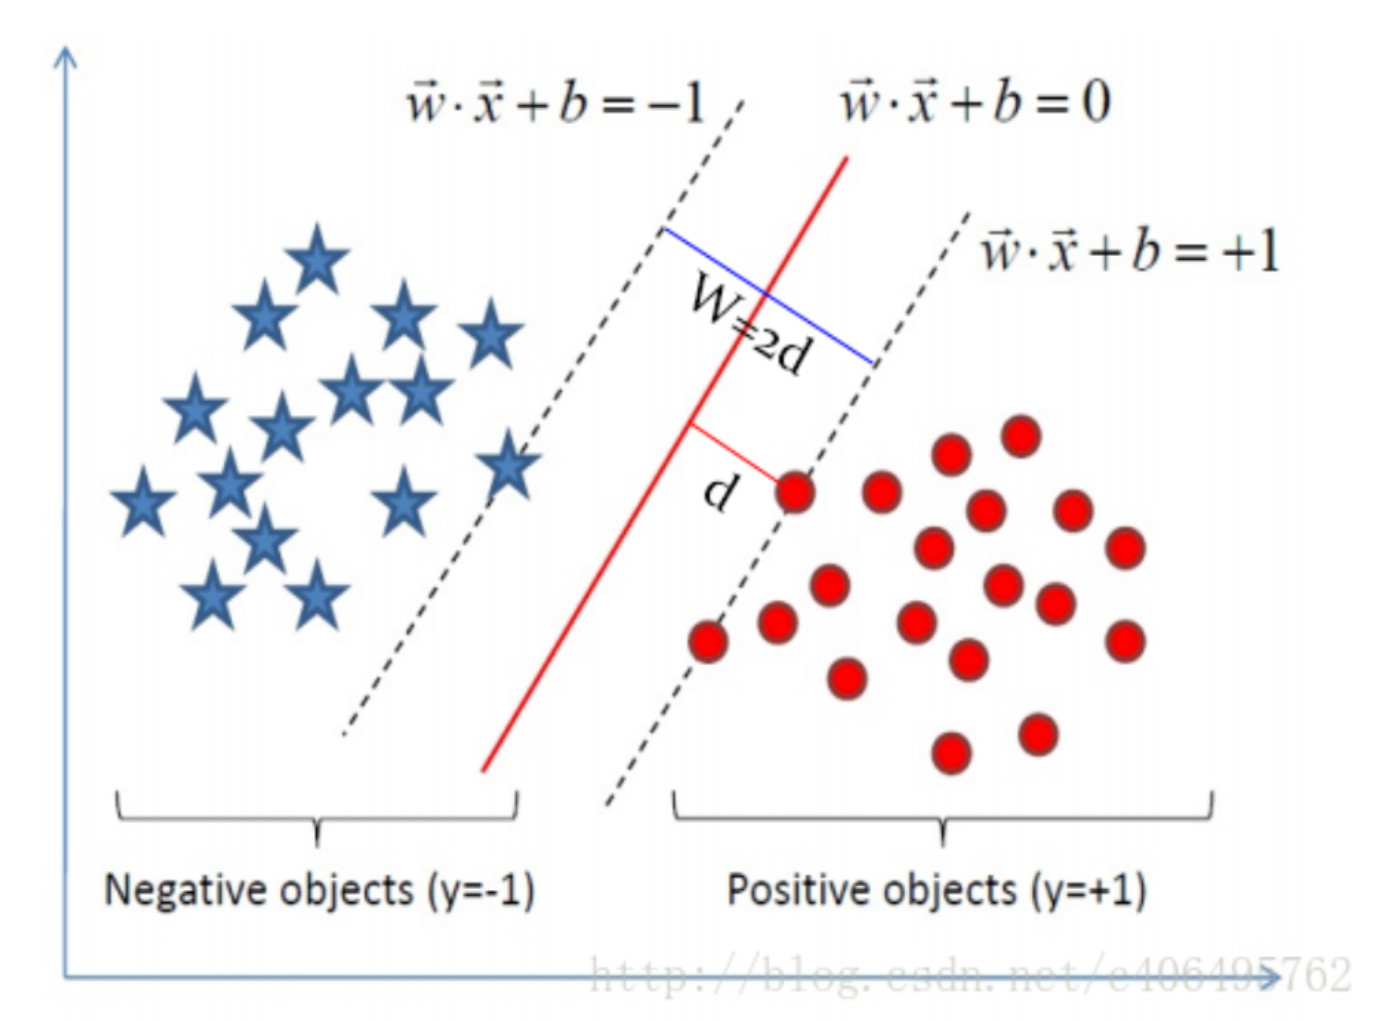
\includegraphics[width=0.6\textwidth]{4.png}
\end{figure}

最后是\textbf{约束条件}的确定。首先要考虑的就是,如何判断超平面是否将样本点正确分类?此外,目标函数本质上是求距离$d$的最大值,要确定约束条件,还必须要找到哪些是“支持向量”。总而言之,对于目标函数$d$的取值范围受到的限制和约束条件的确定,关键问题是如何将其数学化。

以上述平面上的分类问题为例:对任意一点$x_i$,其到最优分类直线的距离为$d_i=\frac{|w^Tx_i+b|}{||w||}$

一方面,如果此时最优分类直线确实实现了分类目标,则所有样本点($y_i$ = 1 or $\textnormal{-}1$)必定都要满足约束($d$ 为最优距离):

\begin{equation}
	d_i=\frac{|w^Tx_i+b|}{||w||}\geq d \Leftrightarrow 
	\begin{cases}
		\frac{w^Tx_i+b}{||w||}\geq d,\ y_i=1\ \\
		\frac{w^Tx_i+b}{||w||}\le-d,\ y_i=-1
	\end{cases}
	\Leftrightarrow \ y_i\bullet\frac{w^Tx_i+b}{||w||}\geq d\ 
	\Leftrightarrow \frac{1}{||w||d}\bullet y_i(w^Tx_i+b)\geq1
\end{equation}

注意到:$w^Tx+b=0$与$\frac{1}{||w||d}\bullet(w^Tx+b)=0$本质上代表同一个超平面,因此上述约束条件可以等价改写为:$y_i(w^Tx_i+b)\geq1$。

另一方面,注意到“支持向量”都是位于最优分类超平面上,即若点${(x}_i,y_i)$为“支持向量”,则必有:$w^Tx_i+b=1$。于是最大化目标函数(“支持向量”到最优分类超平面的间隔),等价于最大化:$\frac{1}{||w||}$,也等价于最小化:$\frac{1}{2}{||w||}^2$。

综上所述,硬间隔SVM的基本数学模型可以描述为如下不等式约束的二次型函数的约束优化问题:
\begin{equation}
	\begin{cases}
		\mathop{min}\limits_{w,b}{{\frac{1}{2}||w||}^{2}}\\                                                   
		st:\ y_i(w^Tx_i+b)\geq1,\ i=1,\cdots,n \\
	\end{cases}
\end{equation}

该优化问题由于受不等式约束,因此求解过程中还需要考察拉格朗日对偶问题和KKT条件。基于不等式约束的凸优化问题,可以基于拉格朗日对偶问题和KKT条件,然后利用\textbf{SMO算法求解},得到最优$w^\ast,b^\ast$,从而可构造最优分类超平面:
\begin{equation}
	{(w^\ast)}^Tx+b^\ast=0
\end{equation}

对待分类的样本点$x$,根据以下决策函数来进行分类判别$f(x)=sgn({(w^\ast)}^Tx+b^\ast)$,即当${(w^\ast)}^Tx+b^\ast>0$时返回0,否则返回1。

基于以上理论,可实现经典硬间隔SVM模型建构。在R语言中,$e1071$程序包内的$svm()$函数是对于经典硬间隔SVM模型的封装实现,其基本用法如下:

\begin{lstlisting}[language=R]
	# 训练 SVM 模型
	model <- svm(formula,data,labels,scale=TRUE/FALSE,kernel,gamma=g,degree=d,cost=C,epsilon=0.1,na.action=na.omit/na.fail)
\end{lstlisting}

其中:
\begin{itemize}
	\setlength{\parsep}{0ex} %段落间距
	\setlength{\topsep}{2ex} %列表到上下文的垂直距离
	\setlength{\itemsep}{1ex} %条目间距
	\item \textbf{formula}:拟合公式,以R公式的形式指定输出变量和输入变量,其格式一般为:输出变量名~输入变量名;		
	\item \textbf{data}:训练数据集(各协变量),通常是一个数据框或矩阵;
	\item \textbf{labels}:标签数据(二元响应变量),通常是一个因子向量,用于指定那些将被用来训练模型的采样数据;
	\item \textbf{scale}:逻辑向量,指定特征数据是否需要标准化(默认标准化为均值0,方差1),默认为True;
	\item \textbf{kernel}:核函数类型,常用的有 "linear"、"polynomial"、"radial" (RBF) 和 "sigmoid";
	\item \textbf{gamma}:用于指定多项式核以及径向基核中的参数,默认gamma是线性核中的常数项,等于1/p(p为特征空间中的维度);
	\item \textbf{degree}:用于指定多项式核中的阶数d;
	\item \textbf{cost}:惩罚参数,用于控制误分类的惩罚程度;
	\item \textbf{epsilon}:用于指定支持向量回归中的带,默认值为0.1;
	\item \textbf{na.action}:用于指定当样本数据中存在无效的空数据时系统应该进行的处理,默认值na.omit表明程序会忽略那些数据缺失的样本;另外一个可选的赋值是na.fail,它指示系统在遇到空数据时给出一条错误信息。
\end{itemize}

硬间隔支持向量机(Hard-Margin SVM)是支持向量机的一种特殊情况,适用于数据完全线性可分的情况。它通过最大化间隔来找到一个分离超平面,使得所有数据点都在间隔之外且没有误分类点。为实现\textbf{经典的硬间隔SVM模型},可以将$svm()$函数的参数如下设置:
\begin{lstlisting}[language=R]
	# 训练硬间隔SVM模型
	library(e1071) # 需要先导入e1071库
	cost_value <- 1e5 # 设置 cost 为一个非常大的值,从而确保没有误分类
	svm_model <- svm(x_train,y_train, type = "C-classification", kernel = "linear", cost = cost_value, scale = FALSE)
\end{lstlisting}

可以通过$summary()$方法查看训练出的模型的信息:

\begin{lstlisting}[language=R]
	summary(svm_model)
	
	Call:
	svm.default(x = x_train, y = y_train, scale = FALSE, type = "C-classification",
	kernel = "linear", cost = cost_value)
	
	Parameters:
	SVM-Type:  C-classification   #模型类别
	SVM-Kernel:  linear   #模型使用的核函数
	cost:  1e+05   #模型确定的约束违反成本
	Number of Support Vectors:  2	( 1 1 )  
	#模型找到的支持向量数量,两类各有一个
	Number of Classes:  2
	Levels:	0 1   #模型中分类的目标类别
\end{lstlisting}

至此已经基于训练集数据完成了经典硬间隔SVM模型的建立与训练过程。

\subsection{基于Logistic回归模型的建模}

与SVM模型类似,Logistic回归模型也旨在研究协变量$X_1,\cdots,X_p$是如何影响响应变量$y$的。但不同的是,Logistic作为广义线性回归模型的一种,本质上还是基于“回归”的基本思想,在多元线性回归的基础上进行调整从而能够处理离散的二元数据。

假定对二元响应变量$y$有$n$次观测:$\ y_i \sim B(1,\mu_i),\ i=1,\cdots,n$

显然其均值方差分别为:${E(y}_i)=\mu_i;\ Var(y_i)=\mu_i(1-\mu_i)$。

同时,对协变量$X_1,\cdots,X_p$也有$n$次观测,且记其线性组合分别为:

$\eta_i=\beta_0+x_{i1}\beta_1+\cdots+x_{ip}\beta_p=x_i^T\beta,\ i=1,\cdots,n$

其中:$x_i={(1,x_{i1},\cdots,x_{ip})}^T, \beta={(\beta_0,\beta_1,\cdots,\beta_p)}^T$

在多元线性回归的过程中,由于响应变量$y$连续,因此可以直接令其均值${E(y})$等于协变量与未知参数的线性组合$\eta$;但对于二元(取值仅存在0或1两种情况)的响应变量而言,这样简单粗暴的处理方式显然是不合适的,需要在原来的方法上做推广,即“广义”的线性回归模型:既然无法直接令两者相等,不妨寻找一个\textbf{链接函数},将多元线性回归中值域为$R$的协变量线性组合$\eta_i=x_i^T\beta$映射到$\mu_i\in(0,1)$区间上,从而便于分类过程的实现。

具体而言,在建立广义线性回归模型的过程中,需要在多元线性回归的基础上选取合适的链接函数$g(\bullet)$把$y_i$的期望$\mu_i={E(y}_i)$和协变量的线性组合$\eta_i=x_i^T\beta$联系起来,使得$g(\mu_i)=\eta_i$。这样的链接函数应该具有良好的性质(如光滑等),才便于后续计算。

针对二元响应变量的分类过程,常用的连接函数为Logistic链接函数:

\begin{equation}
	g(x)=ln{\frac{x}{1-x}},\ x\in(0,1)
\end{equation}

基于Logistic链接函数构造的广义线性回归模型即为Logistic回归模型,其基本内容如下:

\begin{equation} 
	\begin{cases}
		 y_i \sim B(1,\mu_i), i=1,\cdots,n \\
		 g(\mu_i)=\mu_i=x_i^T\beta        
	\end{cases}
\end{equation}

事实上,基于给定的样本数据(训练集数据),训练模型的过程即为对未知参数向量$\beta$进行极大似然估计的过程,但与线性模型不同的是,该模型中极大似然估计并没有显式解,因此需要基于特定的算法进行数值求解,一般采用Newton-Raphson迭代算法,这里不详细展开求解过程。

在R语言中,Logistic模型的训练由基本包中自带的$glm()$函数实现,其基本用法如下:
\begin{lstlisting}[language=R]
	# 训练广义线性模型
	model <- glm(formula, data = mydata, family = family(link = "link_function"))
\end{lstlisting}

其中:
\begin{itemize}
	\setlength{\parsep}{0ex} %段落间距
	\setlength{\topsep}{2ex} %列表到上下文的垂直距离
	\setlength{\itemsep}{1ex} %条目间距
	\item \textbf{formula}:表示响应变量与解释变量的关系公式,如$y \sim x1 + x2$;		
	\item \textbf{data}:所用的数据集(需要为数据框格式来识别特征和标签);
	\item \textbf{family}:表示所拟合的GLM模型类型,包括(但不限于)高斯、二项分布、泊松分布等;
	\item \textbf{link}:表示链接函数,常见的有"identity"、“logit”、"log"等。
\end{itemize}

为实现广义回归模型中的Logistic回归模型,可按照如下方式进行调用:
\begin{lstlisting}[language=R]
	# 将训练数据转换为数据框
	train_data <- data.frame(x = x_train, y = as.factor(y_train))
	
	# 训练Logistic回归模型
	logistic_model <- glm(y ~ ., data = train_data, family = binomial)
\end{lstlisting}

同样采用$summary()$方法查看训练模型的信息:

\begin{lstlisting}[language=R]
	summary(logistic_model)
	
	Call:   # 调用信息, 说明模型使用了二元逻辑回归和所有特征。
	glm(formula = y ~ ., family = binomial, data = train_data)
	
	Coefficients:   # 估计值、标准误差、$z$值和$p$值的表格。
	(Intercept)  -169.33   32205.14  -0.005    0.996
	# 截距项的估计值、标准误差、$z$值和$p$值。
	x.1            15.32    5873.78   0.003    0.998
	# 第一个特征$x.1$的估计值、标准误差、$z$值和$p$值。
	x.2            63.10   13139.18   0.005    0.996
	# 第二个特征$x.2$的估计值、标准误差、$z$值和$p$值。
	(Dispersion parameter for binomial family taken to be 1)
	# 二项分布的离散参数被设定为$1$。
	Null deviance: 3.8815e+02  on 279  degrees of freedom
	# 零偏差:模型中只有截距时的偏差, $279$个自由度。
	Residual deviance: 6.1211e-08  on 277  degrees of freedom
	# 残差偏差:模型拟合后的偏差, $277$个自由度。
	AIC: 6	# $AIC$ 值(信息准则), 用于模型选择。
	Number of Fisher Scoring iterations: 25   
	# $Fisher$评分算法的迭代次数。
\end{lstlisting}

至此已经基于训练集数据完成了Logistic回归模型的建立与训练过程。

\subsection{二者分类效果的比较}

前文在生成模拟数据的过程中提到,若生成时设置的正态总体均值差异不同,其聚集效果也会不同,在默认方差为1的情况下,设置均值为0和1的数据点区分不明显,而设置均值为0和5的数据点区分明显。在模型效果测试中,为保证模型聚合等多方面因素,分别选用均值为0和1(数据点区分不明显),以及均值为0和2.8的数据(数据点区分明显)进行模型训练与性能测试。

首先是选用均值为0和1的数据,即标签为0的数据应聚集在点$(0,0)$附近,标签为1的数据应聚集在点$(1,1)$附近。将训练好的模型应用于测试集上并计算其分类准确率,同时绘制其分类结果与分类器效果图像:

\begin{lstlisting}[language=R]
	# 使用SVM模型进行预测
	svm_predictions <- predict(svm_model, x_test)
	# 计算SVM模型的分类准确率
	svm_accuracy <- sum(svm_predictions == y_test) / length(y_test)
	
	# 使用Logistic回归模型进行预测
	logistic_probabilities <- predict(logistic_model, newdata = data.frame(x = x_test), type = "response")
	logistic_predictions <- ifelse(logistic_probabilities > 0.5, 1, 0)
	# 计算Logistic回归模型的分类准确率
	logistic_accuracy <- sum(logistic_predictions == y_test) / length(y_test)
\end{lstlisting}

\begin{figure}[H]
	\centering
	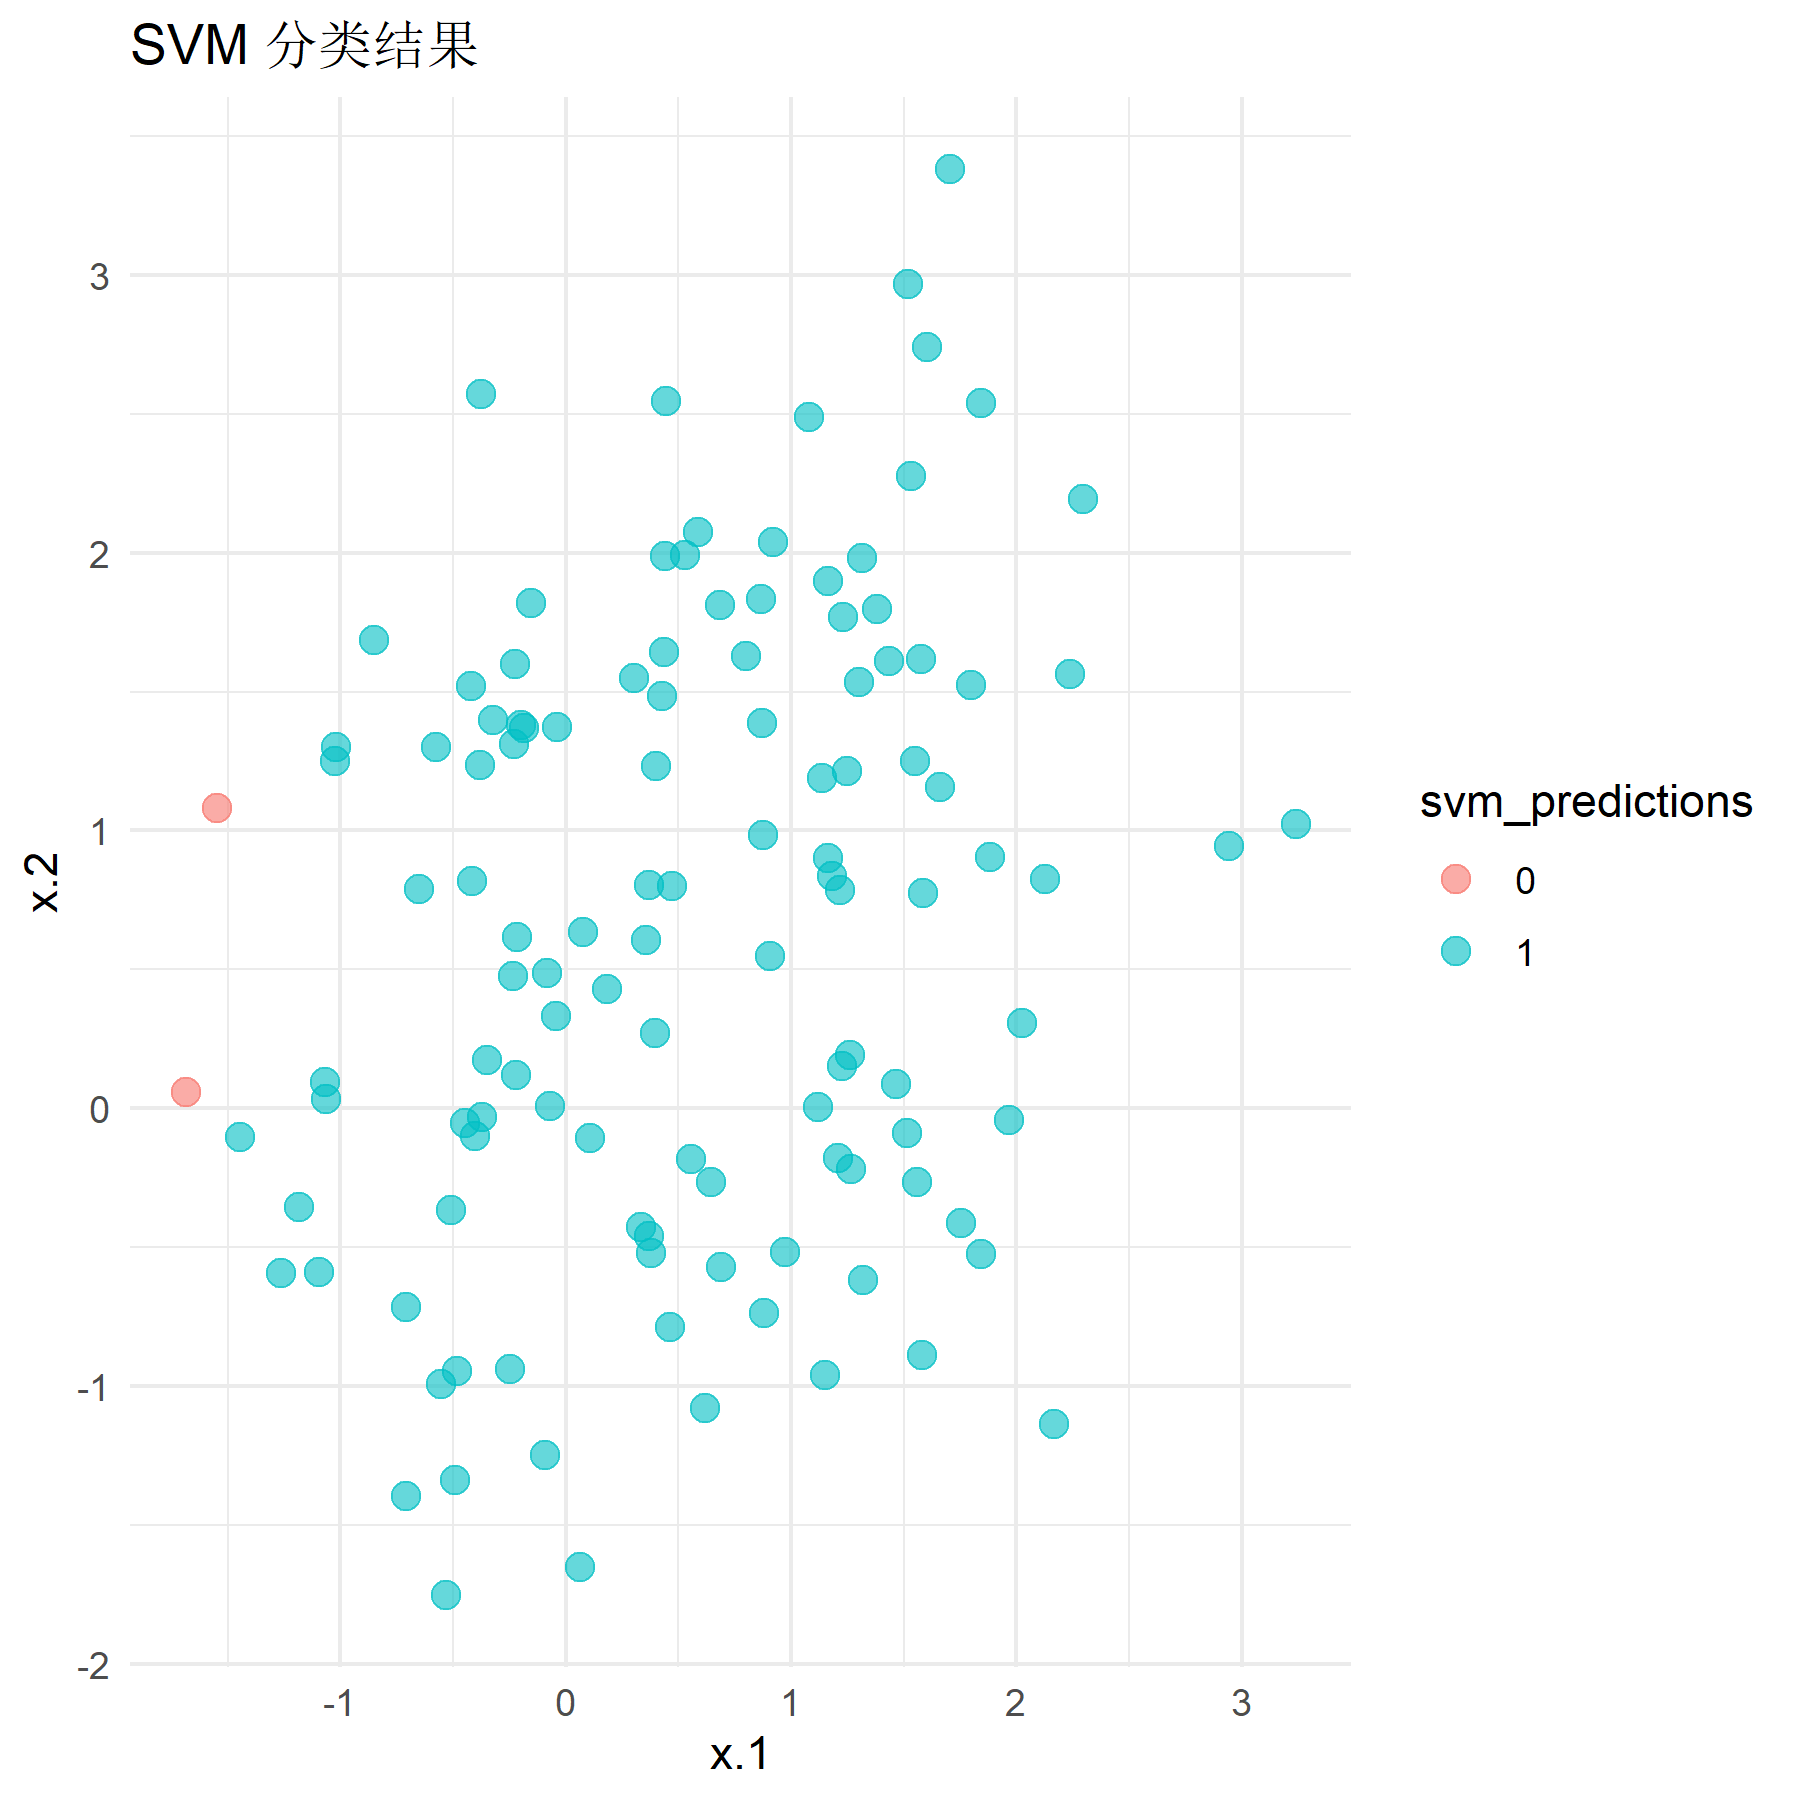
\includegraphics[width=0.25\textwidth]{5.png}
	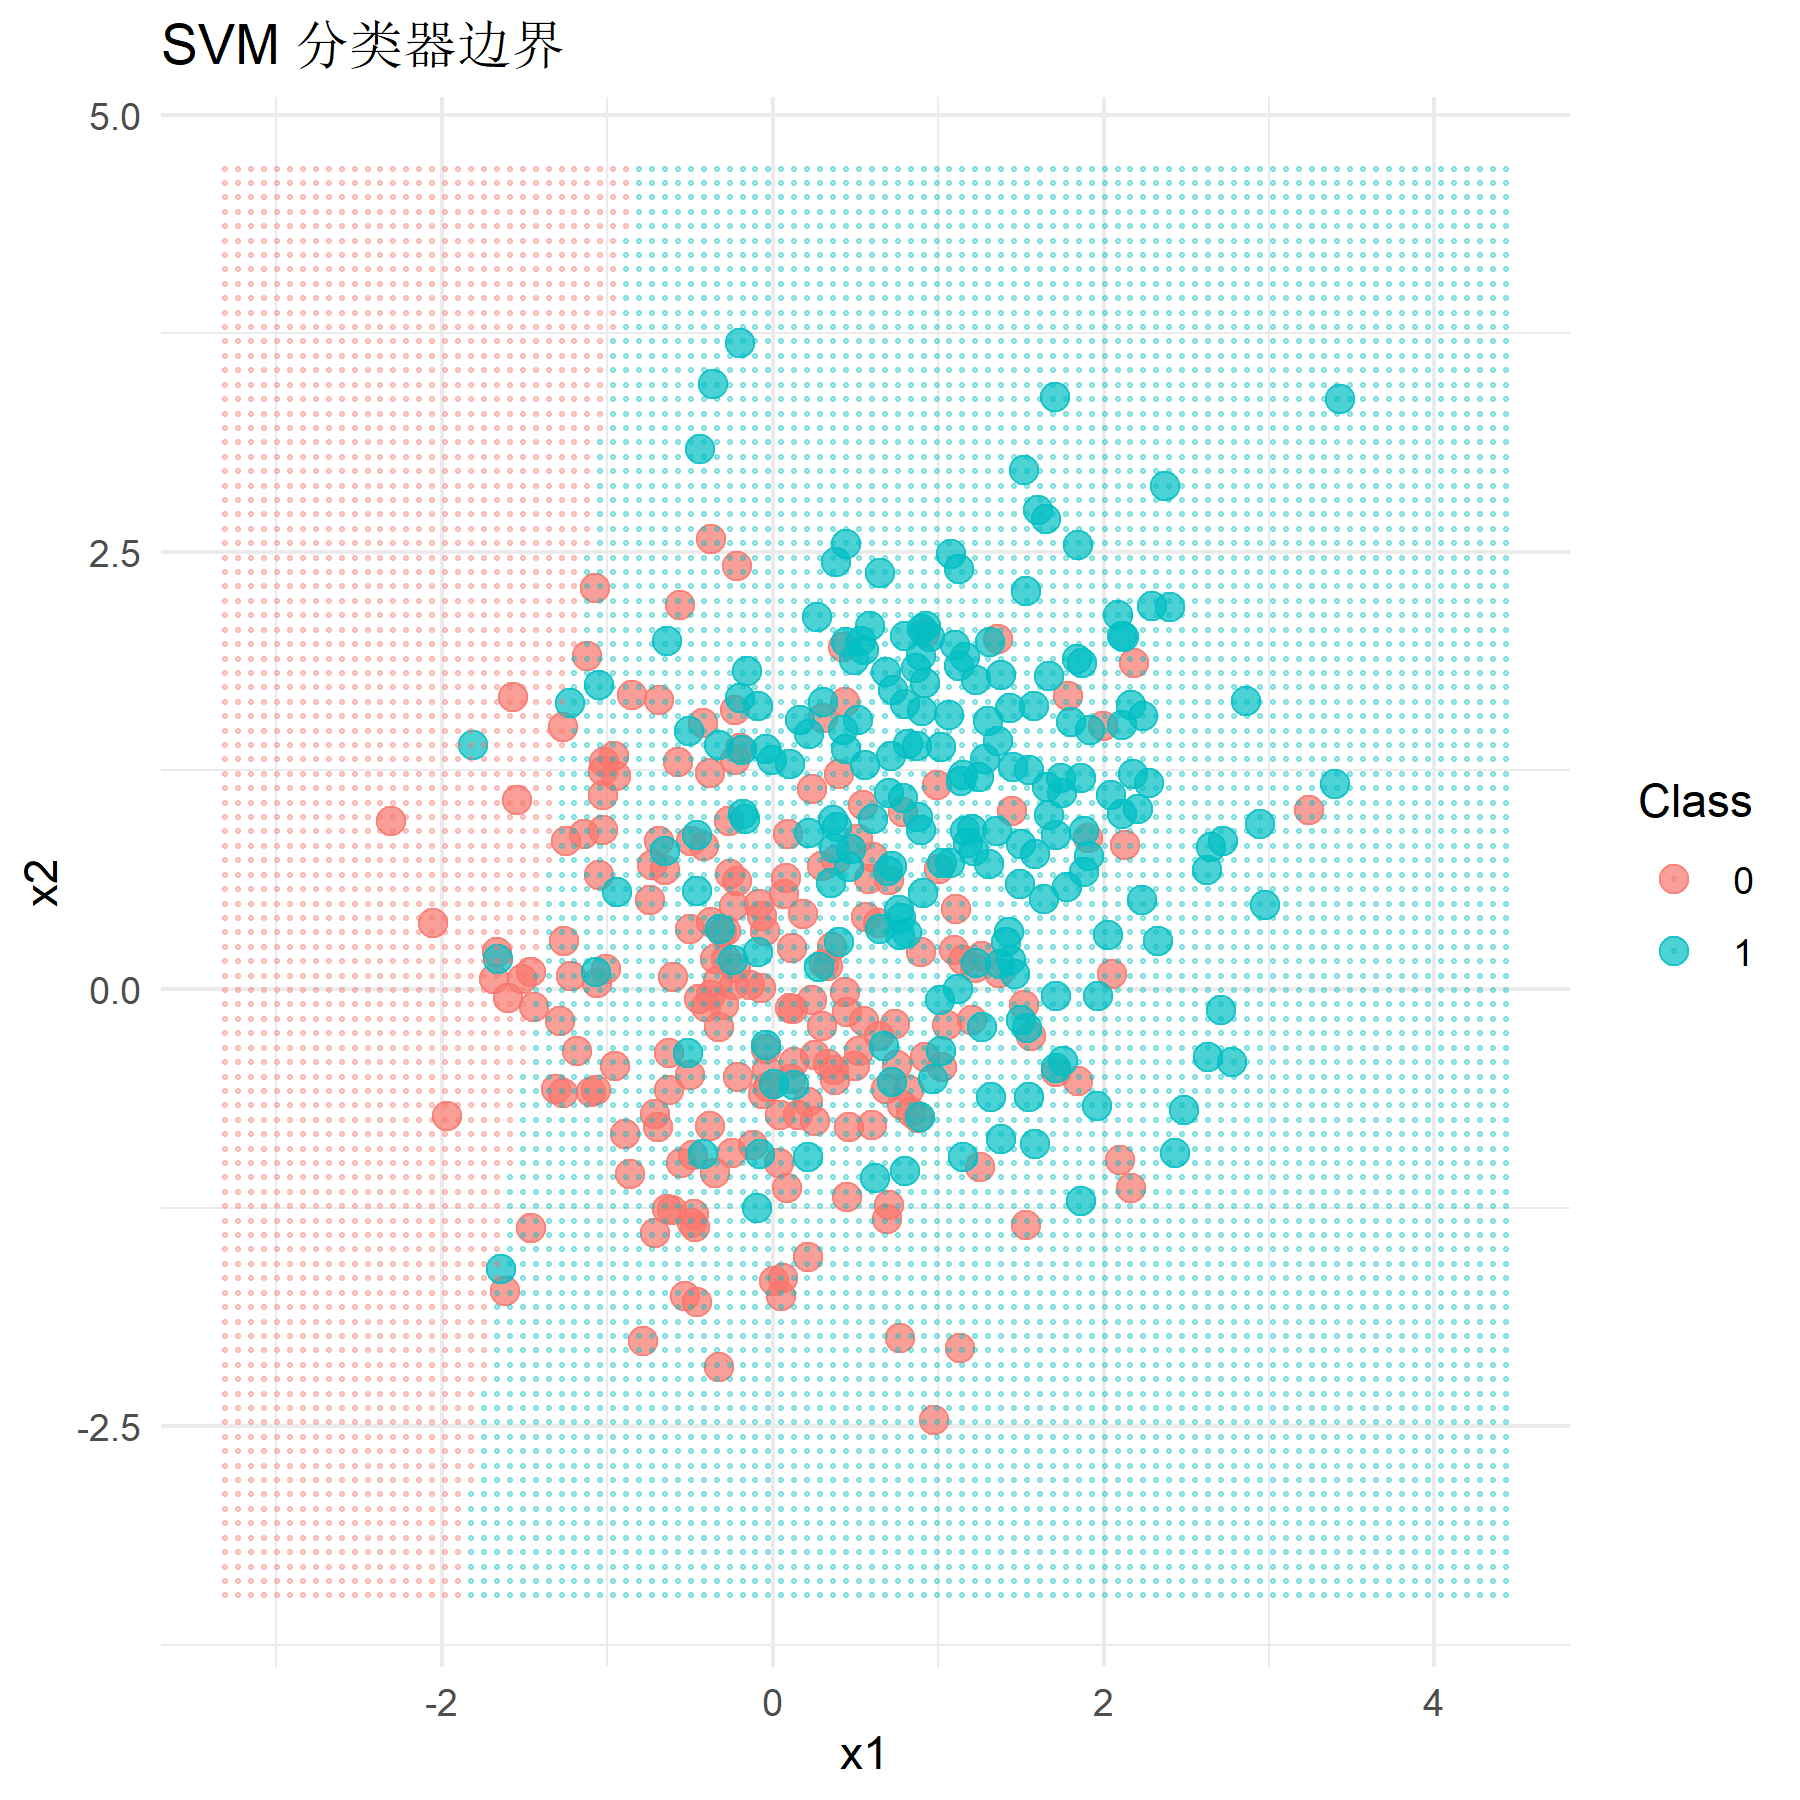
\includegraphics[width=0.25\textwidth]{6.png}
	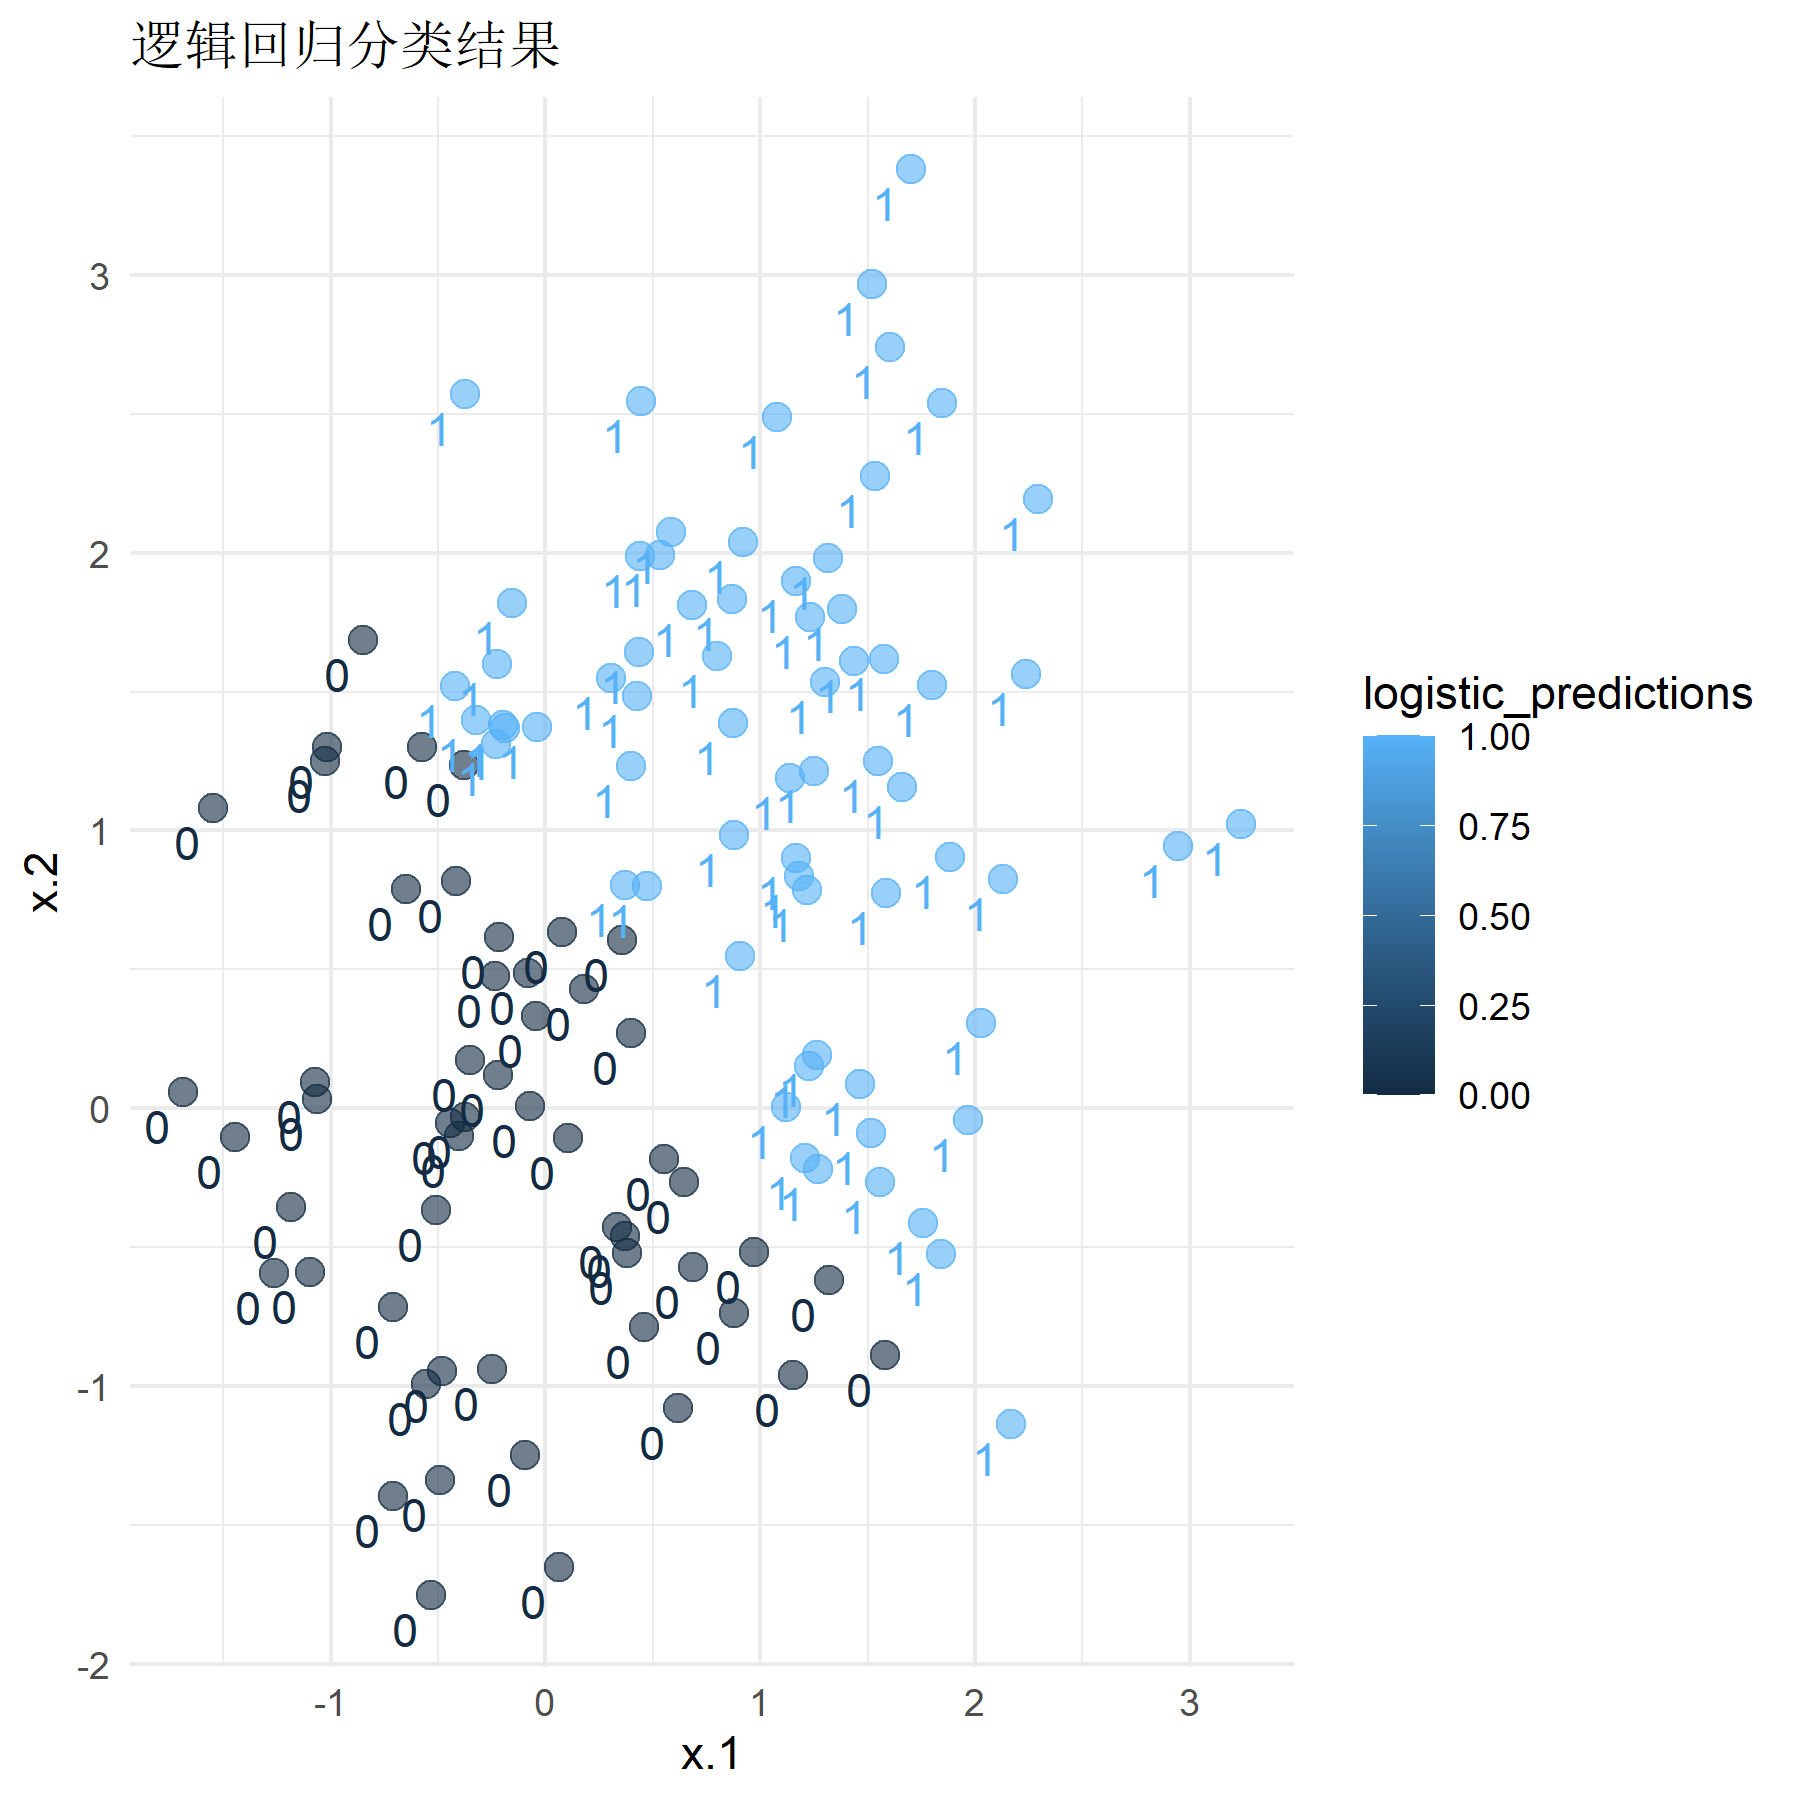
\includegraphics[width=0.25\textwidth]{7.png}
\end{figure}

运行程序,得到该情况下\textbf{SVM模型的分类准确率为0.525},\textbf{Logistic回归模型的分类准确率为0.767}。结合观察图像可知,此时对于\textbf{区分不明显的数据},\textbf{两个模型的分类效果都较差}(90\%以下),但\textbf{Logistic回归模型在数据区分不明显的情况下分类性能要明显优于经典硬间隔SVM模型}。

然后选用均值为0和2.8的数据,即标签为0的数据应聚集在点$(0,0)$附近,标签为1的数据应聚集在点$(2.8,2.8)$附近。将训练好的模型应用于测试集上并计算其分类准确率,同时绘制其分类结果与分类器效果图像:

\begin{figure}[H]
	\centering
	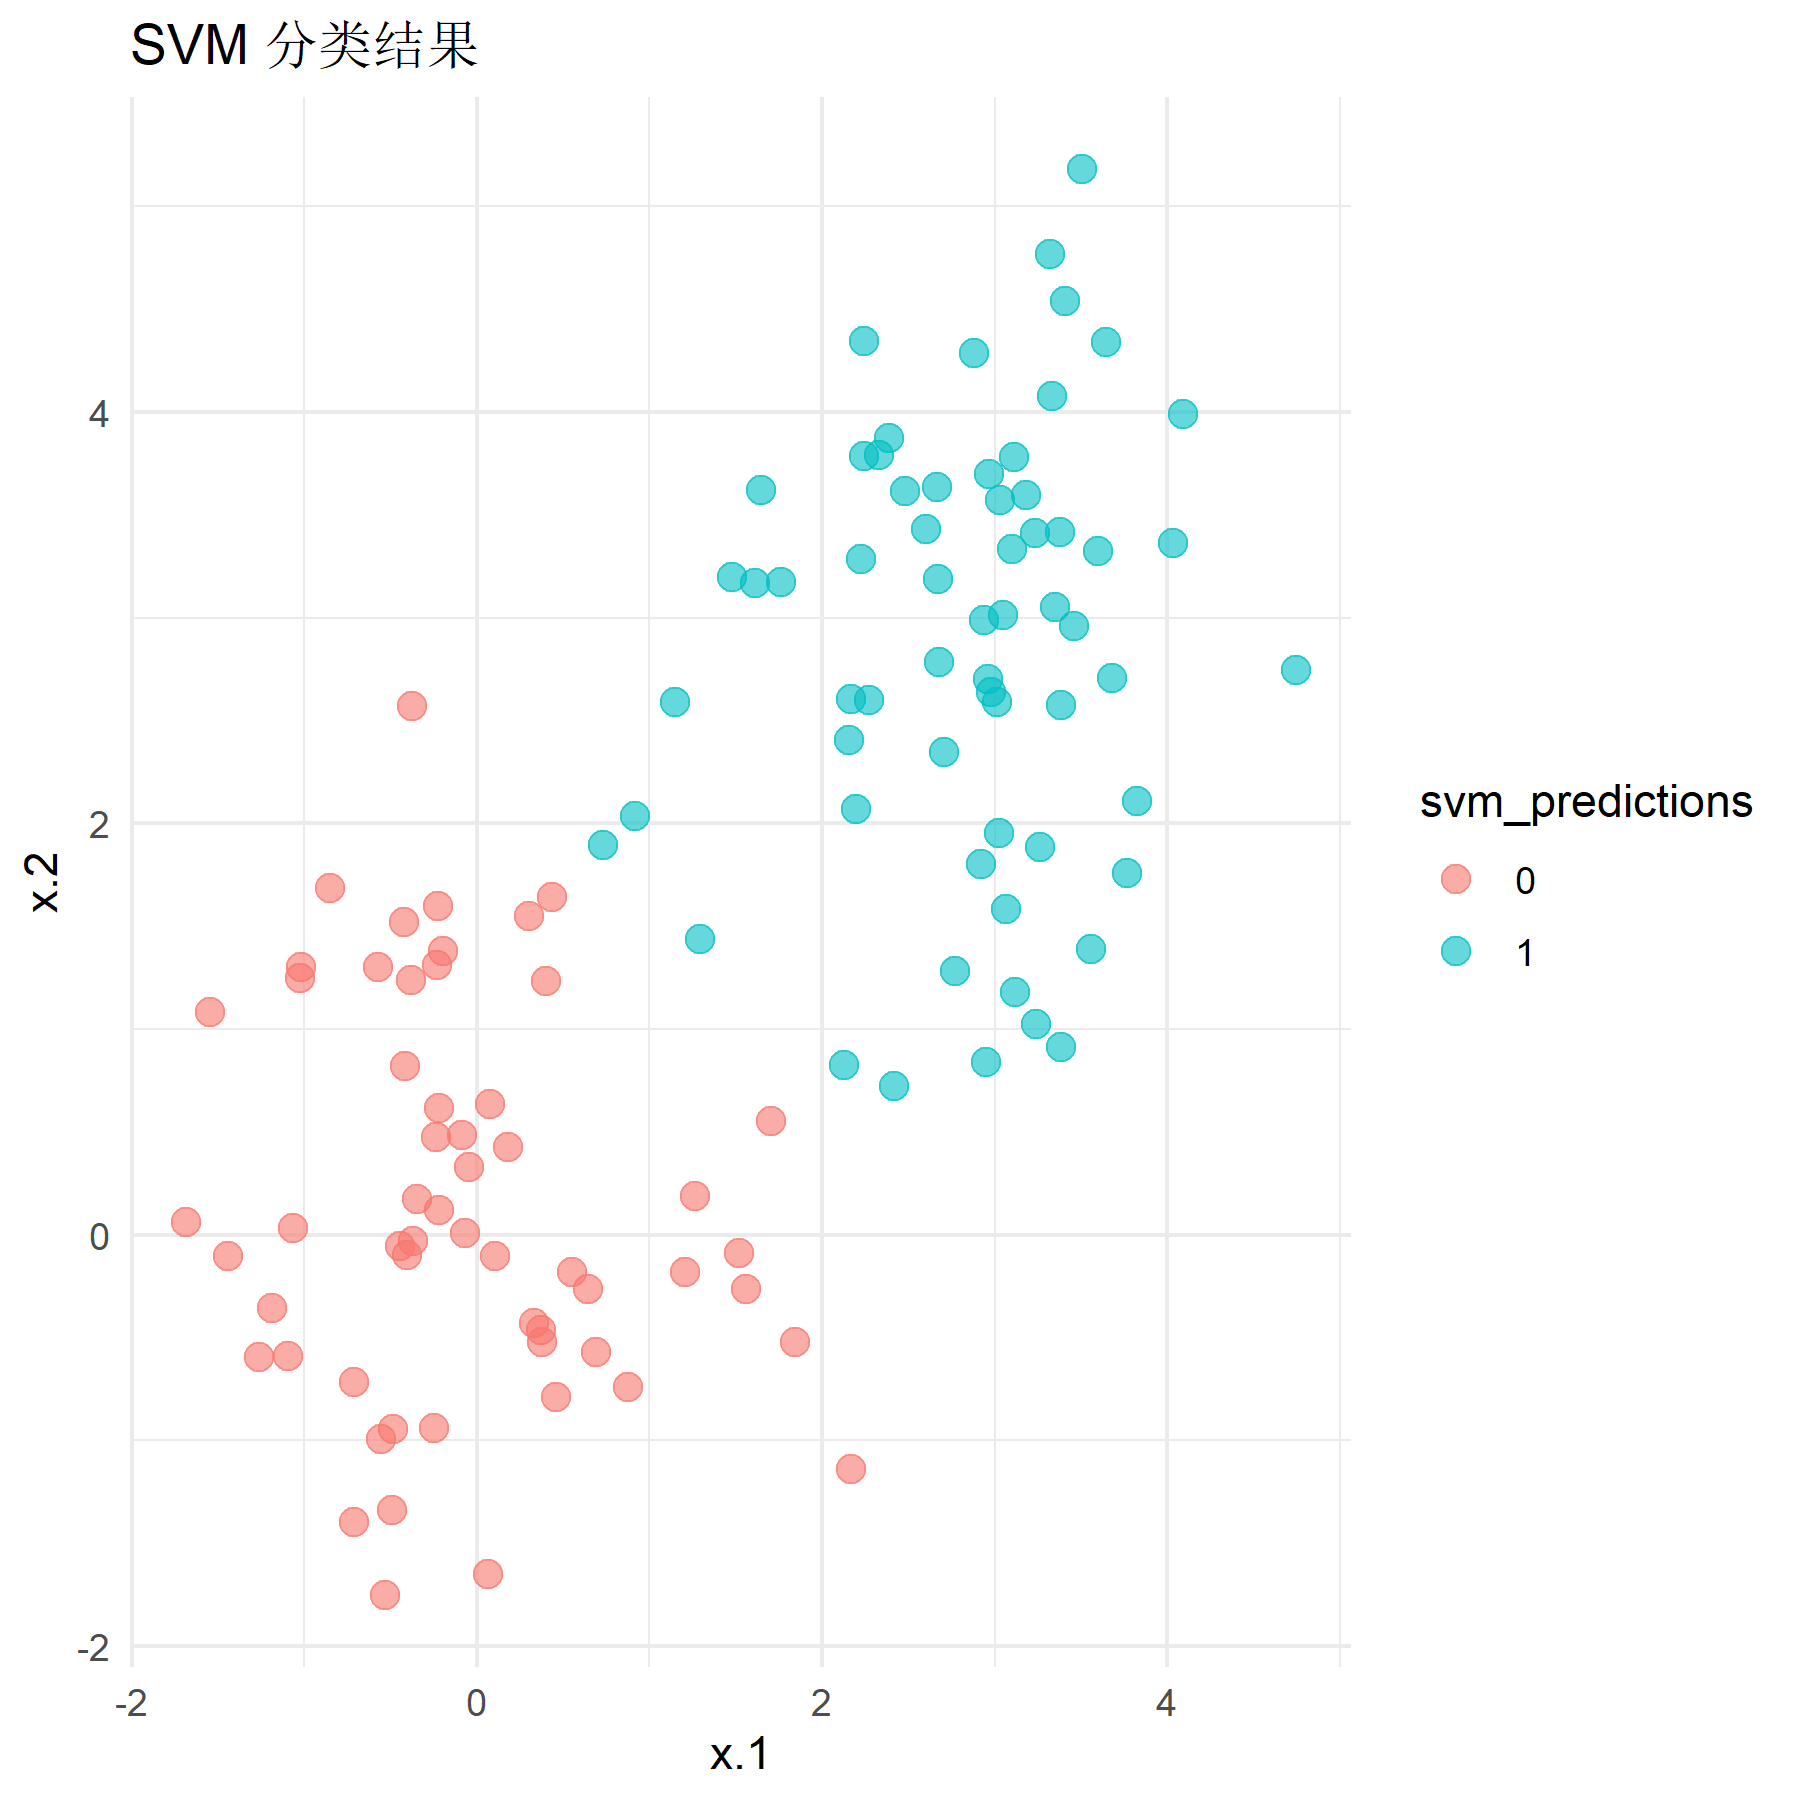
\includegraphics[width=0.25\textwidth]{8.png}
	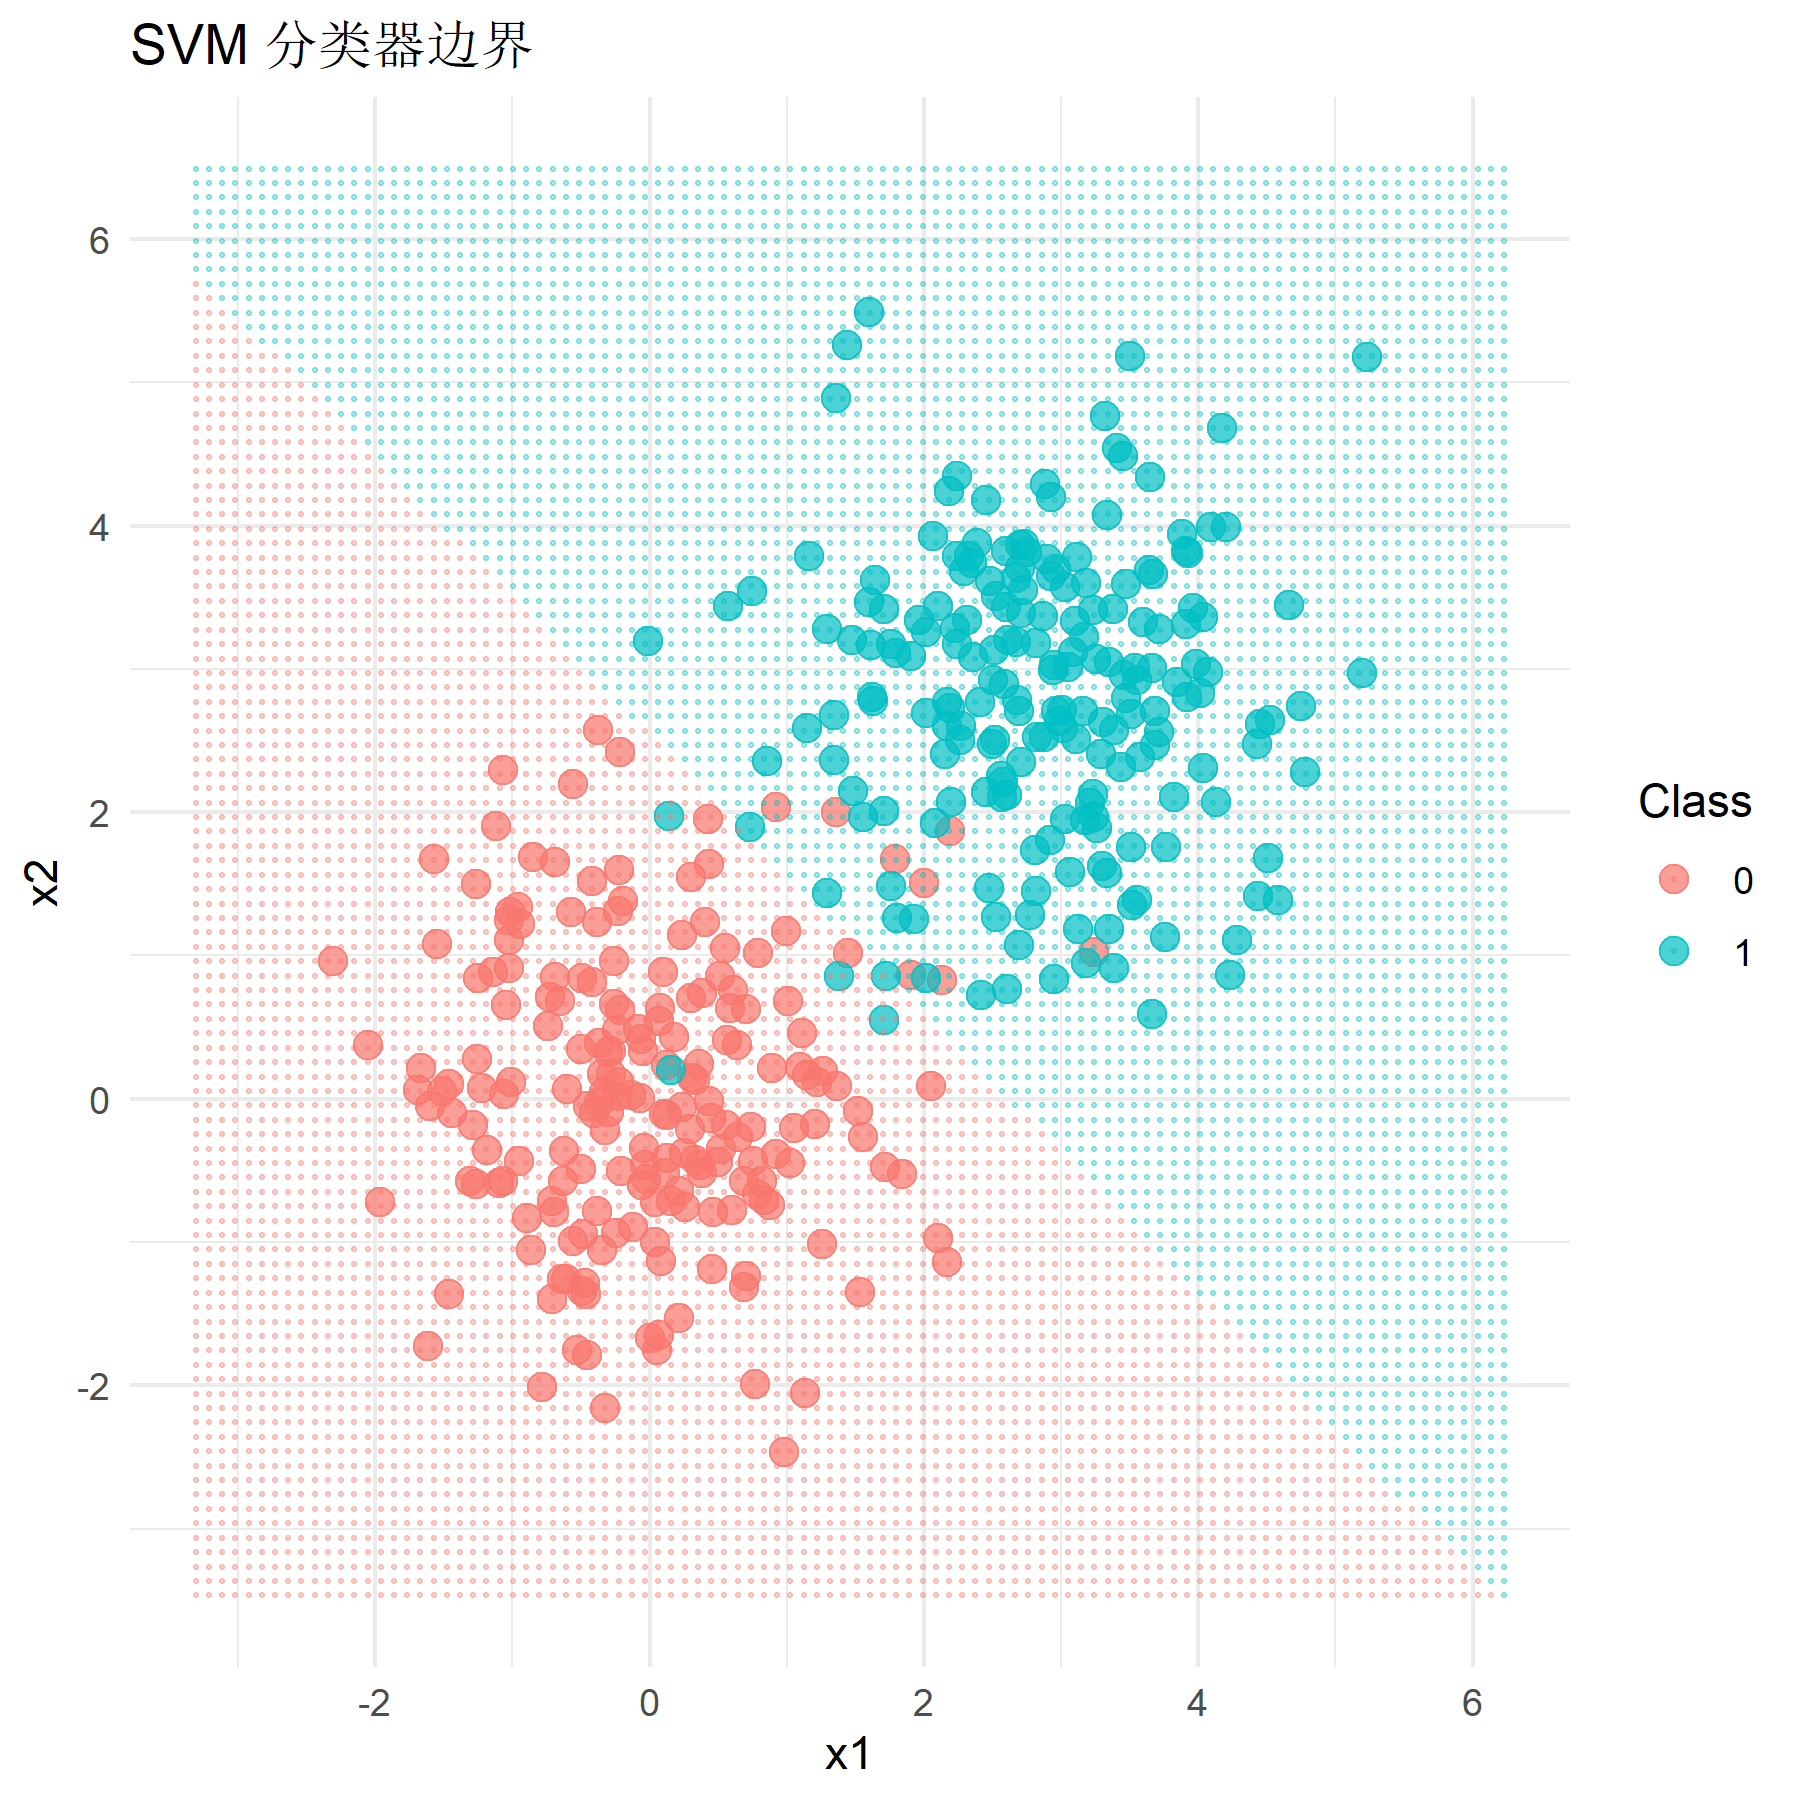
\includegraphics[width=0.25\textwidth]{9.png}
	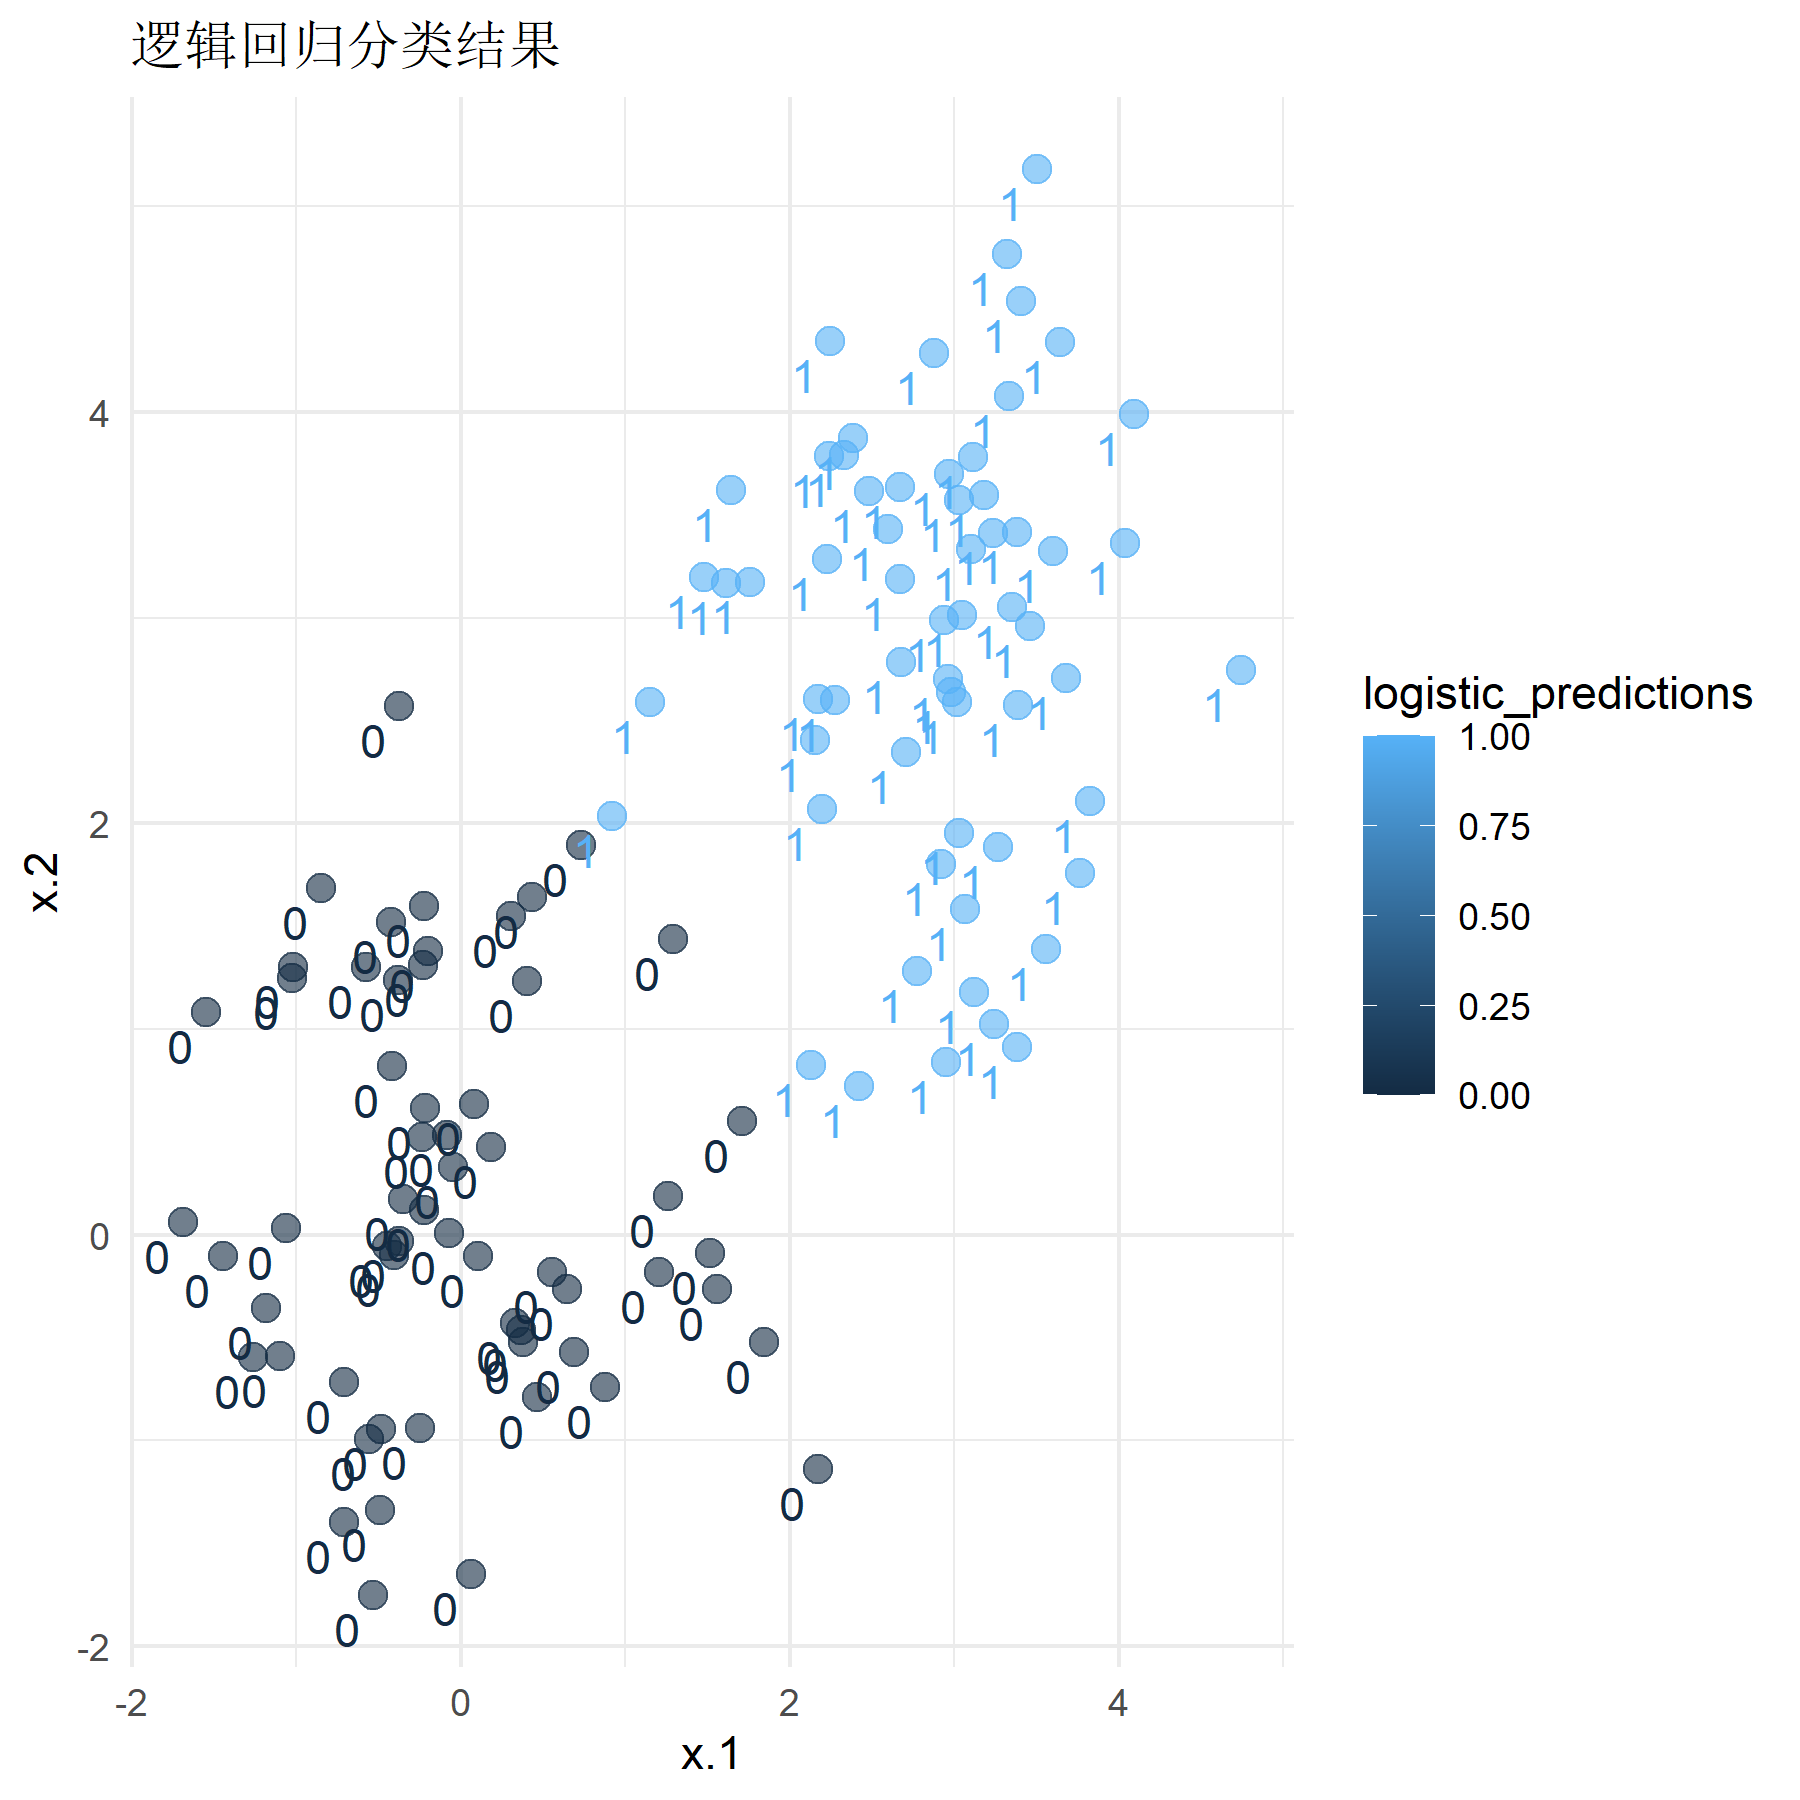
\includegraphics[width=0.25\textwidth]{10.png}
\end{figure}

运行程序,得到该情况下\textbf{SVM模型的分类准确率为0.967},\textbf{Logistic回归模型的分类准确率为0.950}。结合观察图像可知,此时对于\textbf{区分较明显的数据},\textbf{两个模型的分类效果都较好}(90\%以上),但\textbf{经典硬间隔SVM模型在数据区分较明显的情况下分类性能会略优于Logistic回归模型},但总体而言差异并不是很大。

\subsection{改进后SVM模型的性能测试}

上述内容中用到的经典硬间隔SVM模型实际上对于数据有着较高的要求,其实现依赖于样本数据为线性可分这一假设条件,但现实中的实际数据往往很难满足这一点,这也是其缺陷所在。针对不是线性可分的数据,Cortes和Vapnik采用了一种非常巧妙的方式进行改进,即借助函数映射,将低维数据映射到高维空间中,使得在低维空间原来不能线性可分的数据,在高维空间变得线性可分,且可以证明这样的映射始终存在。

\begin{figure}[H]
	\centering
	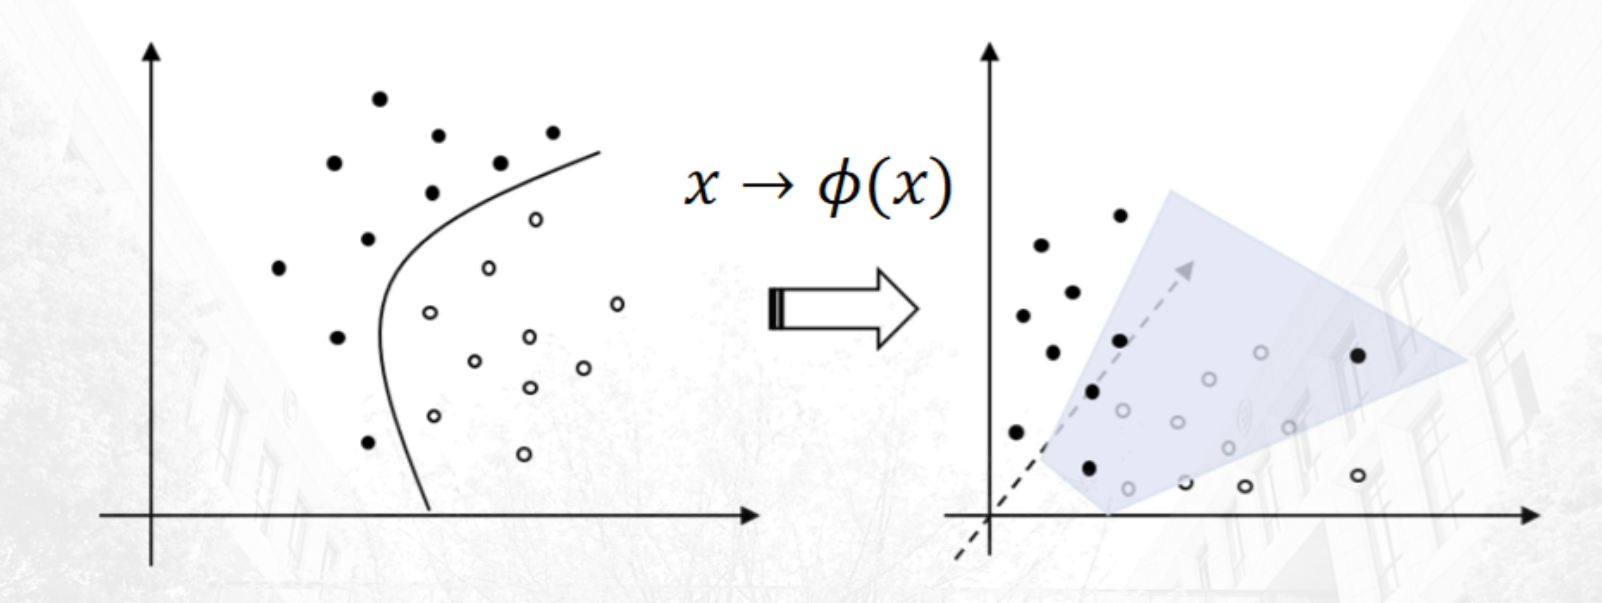
\includegraphics[width=0.6\textwidth]{11.png}
\end{figure}

具体而言,构造升维函数:

\begin{equation}
	K(x,z)=\varphi(x)\bullet\varphi(z)                              
\end{equation}

并构造相应的非线性SVM: 

\begin{equation}
	\begin{cases}
		\mathop{min}\limits_{w,\ b,\ \delta_i} {{\frac{1}{2}||w||}^2}         \\                                           
		st:\ y_i(w^TK(x_i,z)+b)\geq1,\ \ i=1,\cdots,n
	\end{cases}                               
\end{equation}

相应的最优分类超平面为:

\begin{equation}
	{(w^\ast)}^TK(x_i,z)+b^\ast=0
\end{equation}

这里选择\textbf{高斯函数(径向基函数RBF)}作为核函数,将每一个样本点映射到一个无穷维的特征空间从而实现降维,构造改进的SVM模型:

\begin{equation}
	K(x, x') = \exp\left(-\gamma \| x - x' \|^2\right)
\end{equation}

高斯核函数实现的\textbf{功能}是:先将原始的数据点$(x, y)$映射为新的样本$(x',y')$, 再将新的特征向量点乘$(x' . y')$,返回其点乘结果。其主要\textbf{目的}是找到更有利分类任务的新的空间,\textbf{本质}是在衡量样本和样本之间的“相似度”,在一个刻画“相似度”的空间中,让同类样本更好的聚在一起,进而线性可分。

在R语言中,要实现高斯核函数,仅需将调用的$svm()$函数中的参数进行改变:

\begin{lstlisting}[language=R]
	# 训练改进后的非线性SVM模型
	svm_model_modify <- svm(x_train,y_train, type = "C-classification", kernel = "radial", gamma = 2, cost = 1, scale = FALSE)
\end{lstlisting}

其中核函数类型的参数$kernel$由原先的线性函数$"linear"$更换为高斯核函数$"radial"$,并对核函数中的参数$gamma$以及控制误分类的惩罚参数$cost$进行了相应调整。

在\textbf{样本数据区分不明显}(即总体均值设置为0和1)的情况下,运行程序,得到\textbf{改进后的非线性SVM模型的分类准确率为0.767},与Logistic回归模型在该样本下的分类准确率一致,\textbf{较原先经典硬间隔SVM的预测准确率0.525有显著提升}。改进后模型的分类效果如下图所示。

\begin{figure}[H]
	\centering
	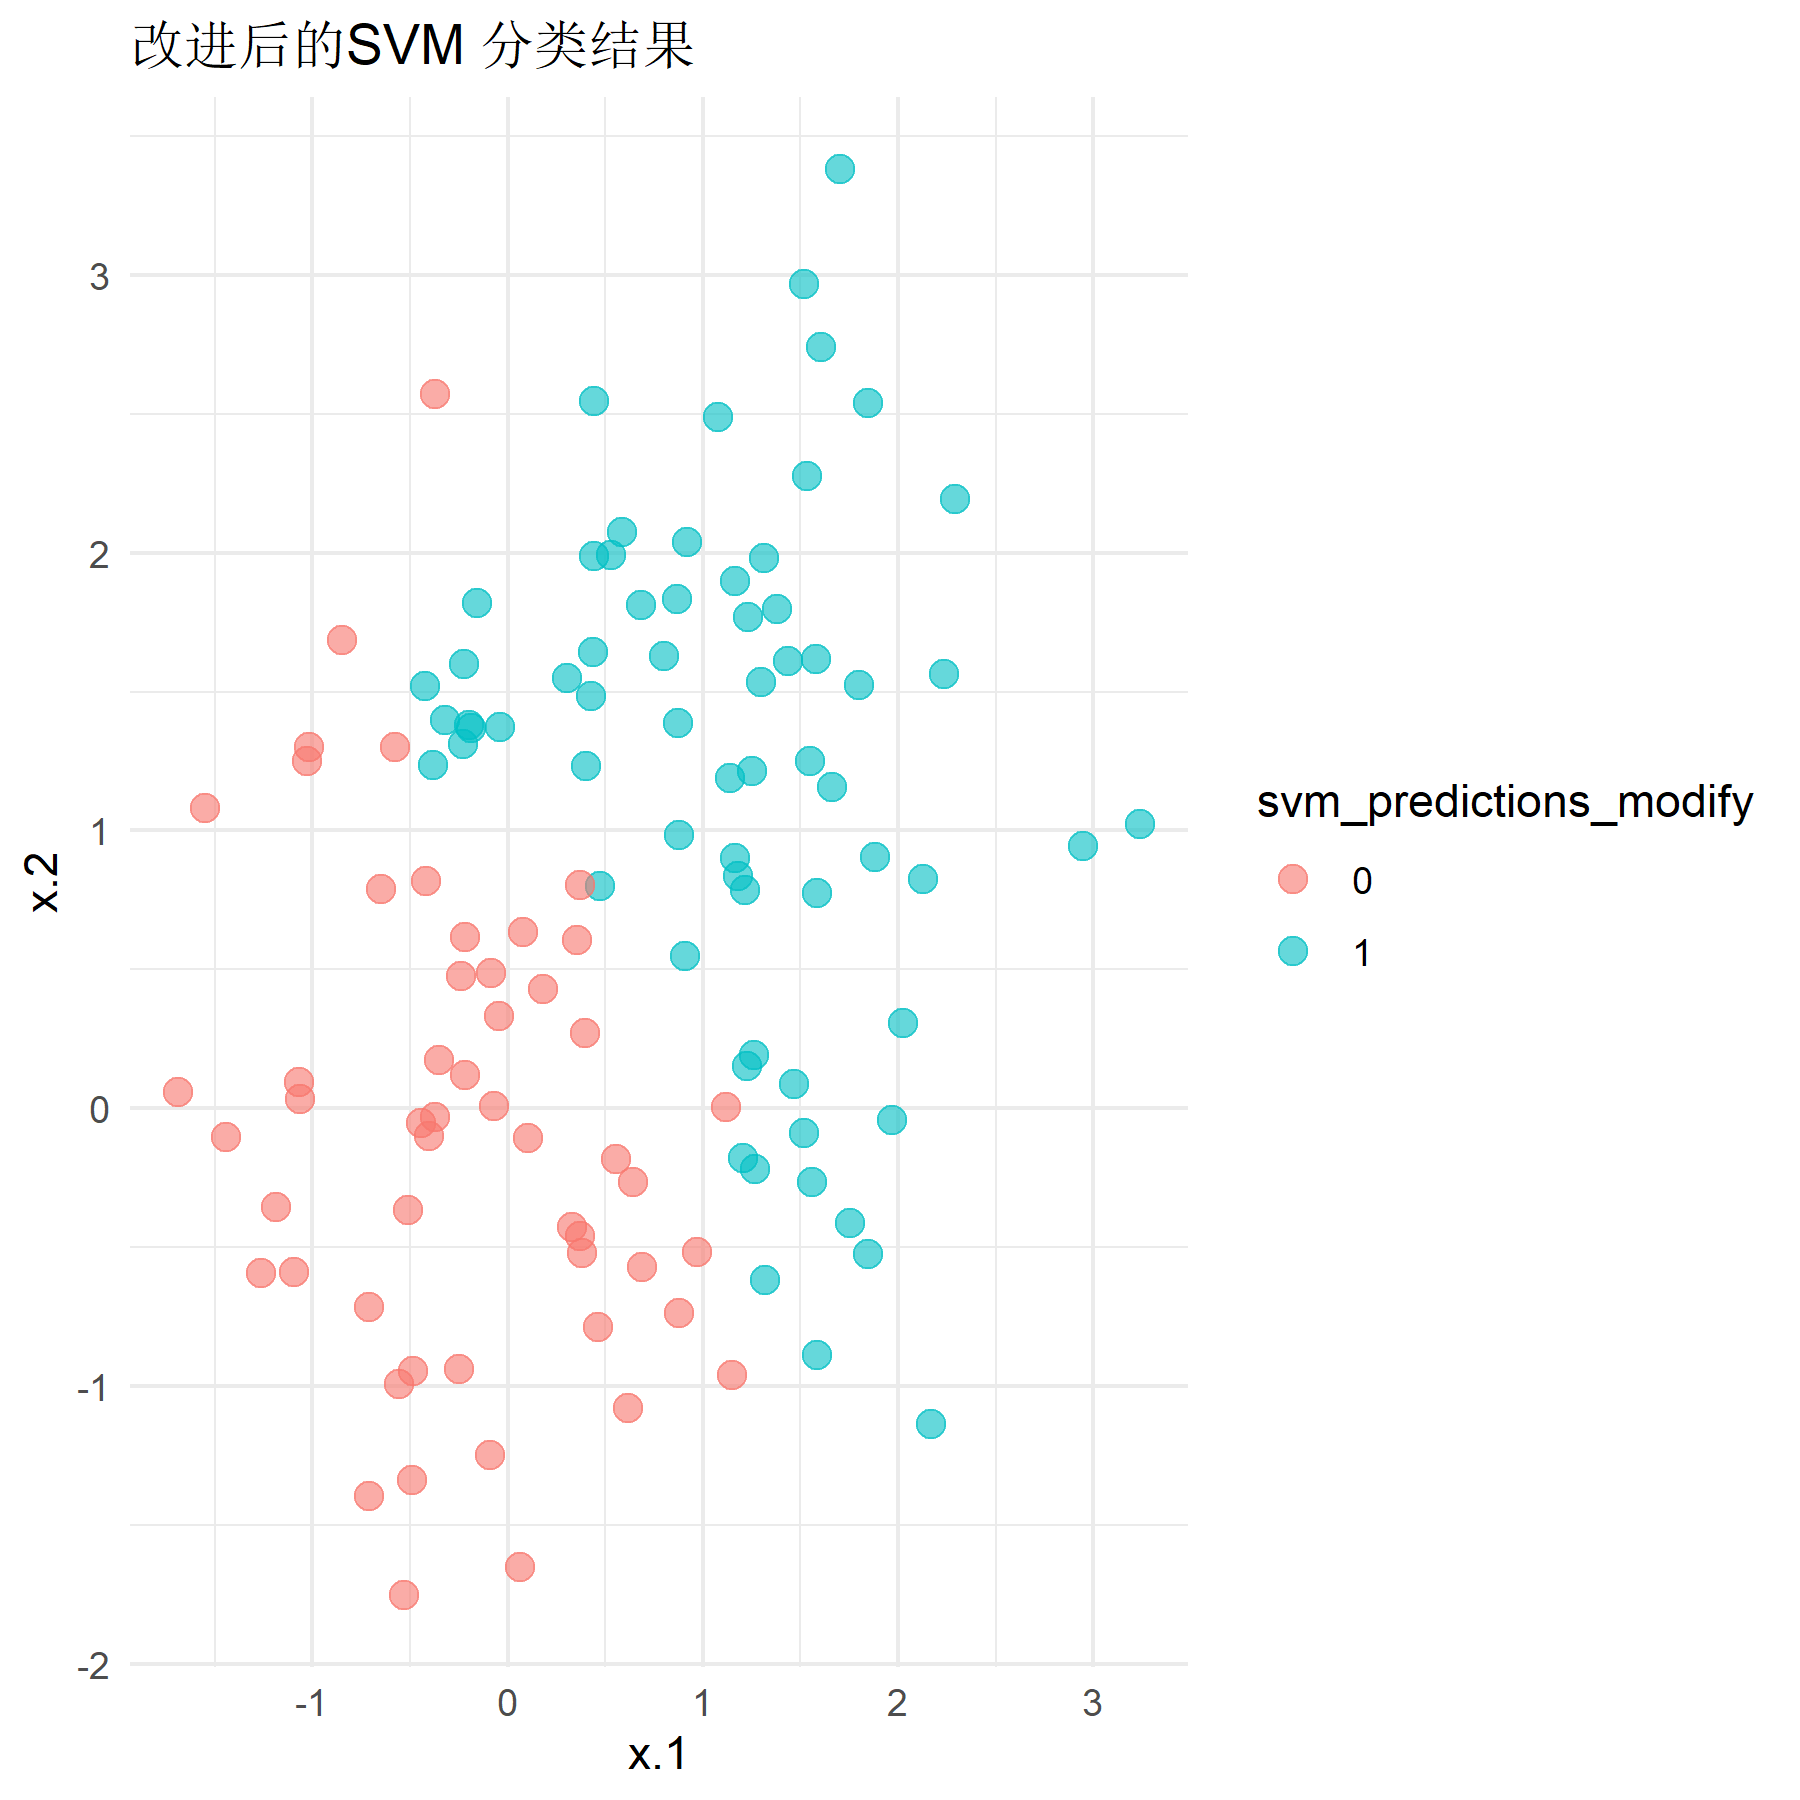
\includegraphics[width=0.4\textwidth]{14.png}
	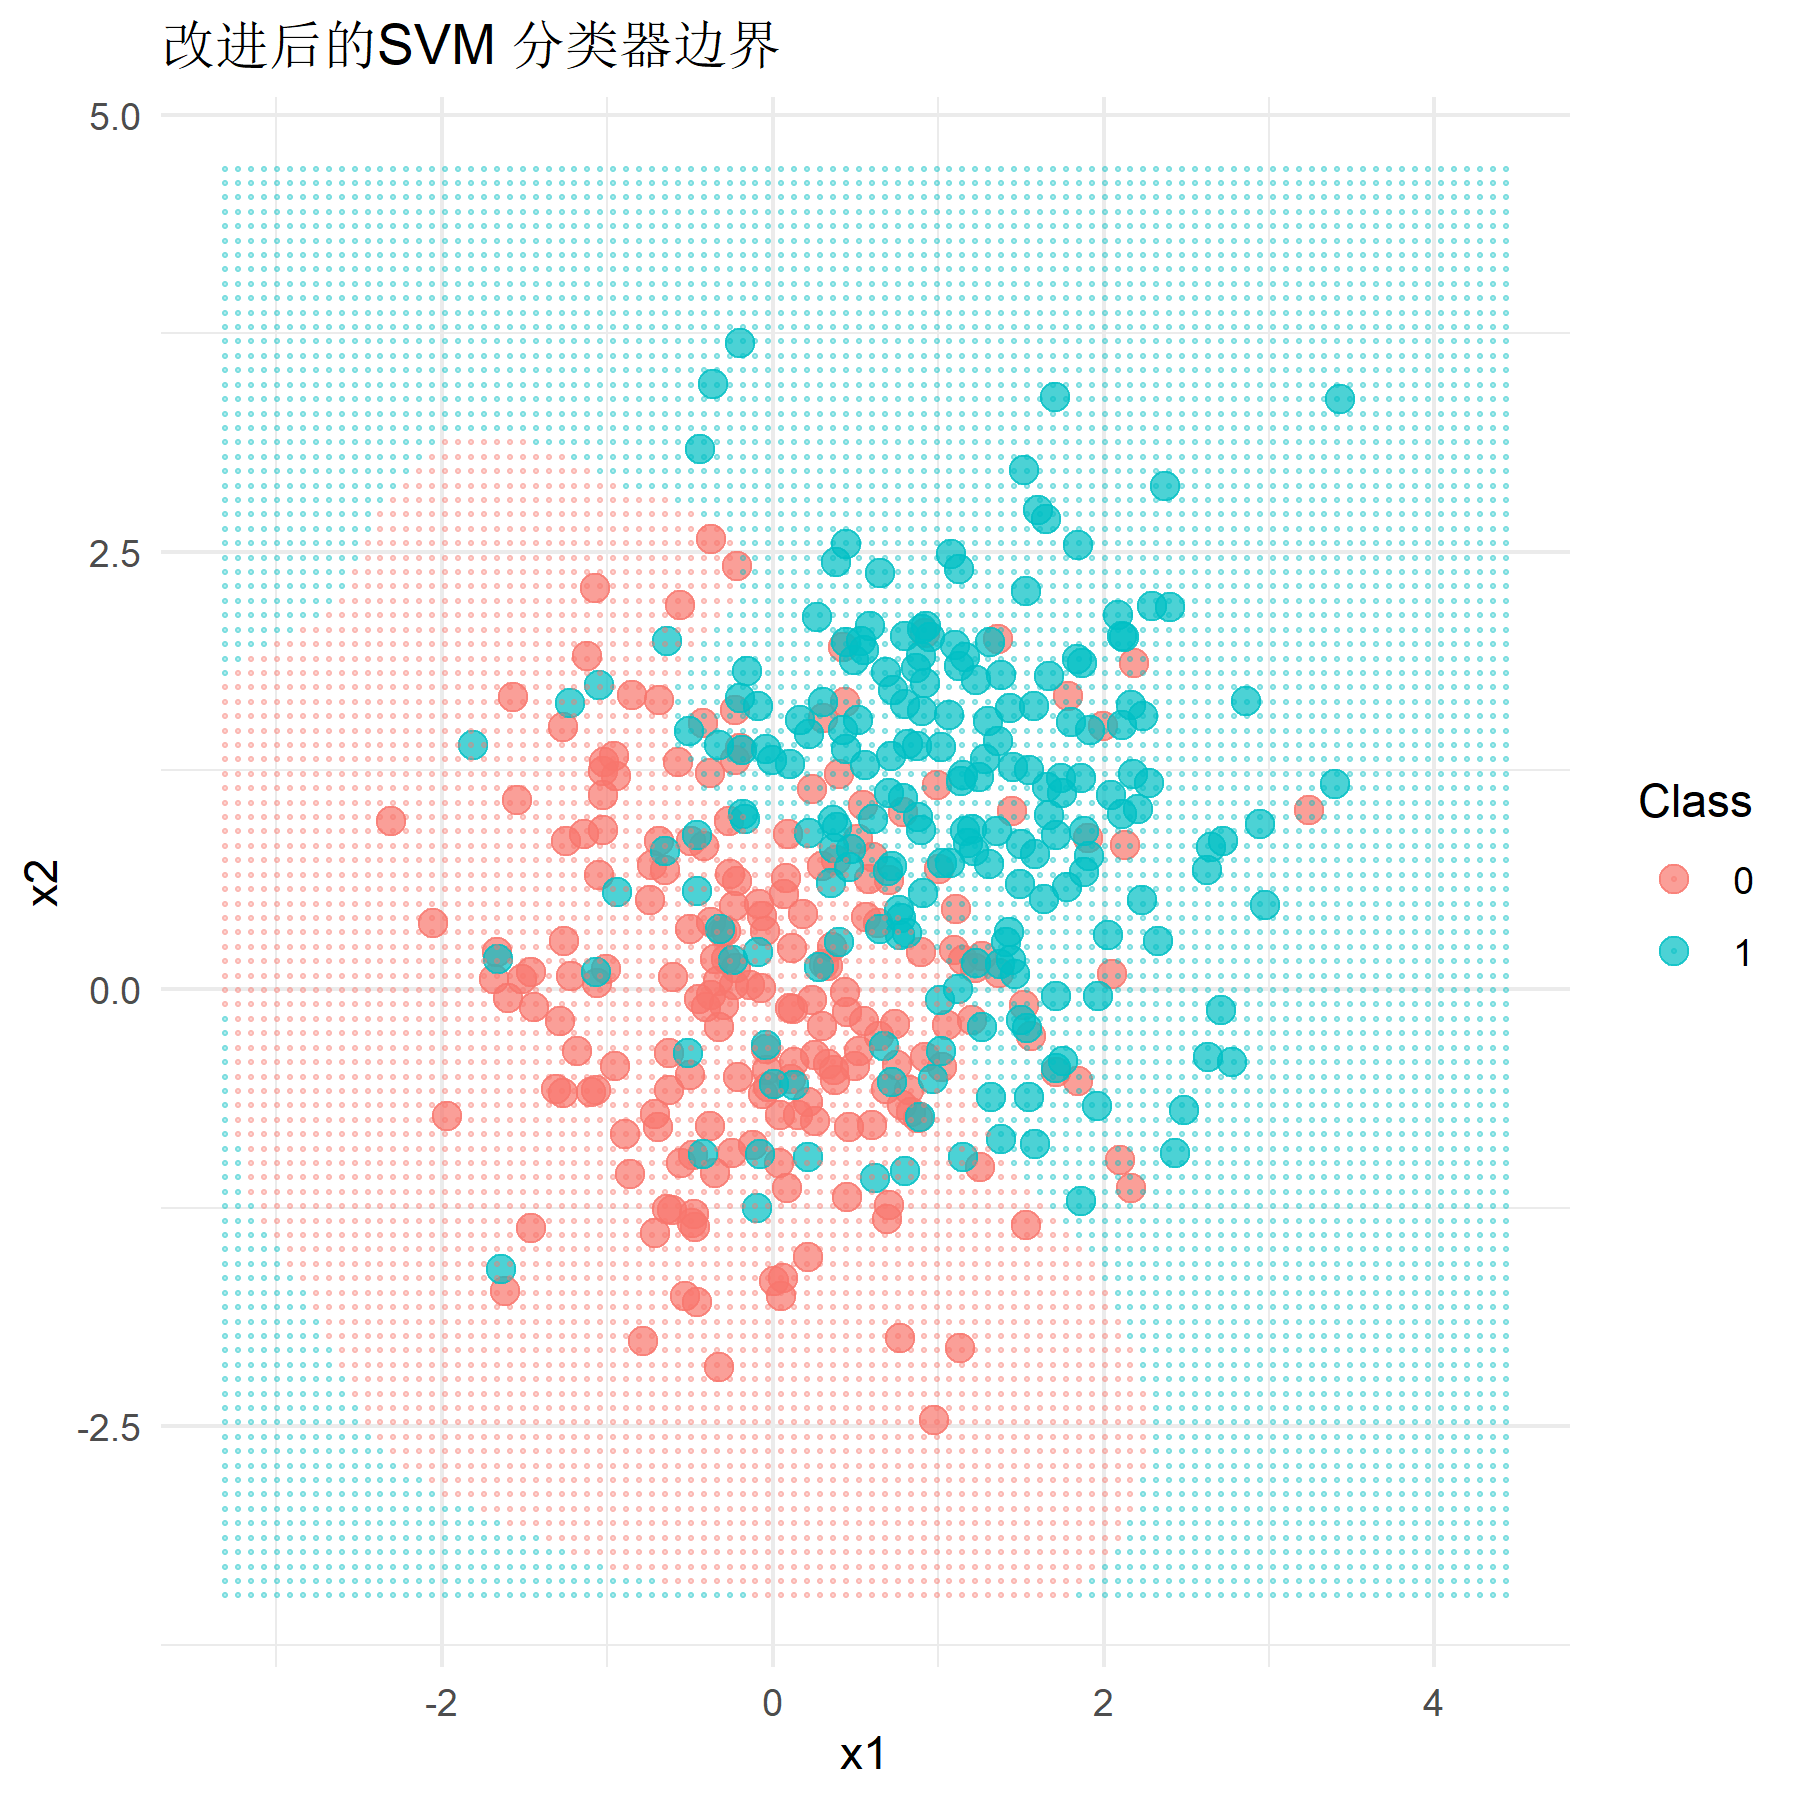
\includegraphics[width=0.4\textwidth]{15.png}
\end{figure}

在\textbf{样本数据区分较明显}(即总体均值设置为0和2.8)的情况下,运行程序,得到\textbf{改进后的非线性SVM模型的分类准确率为0.958},虽然仍优于Logistic回归模型在该样本下的分类效果,但\textbf{较原先经典硬间隔SVM的预测准确率0.967有略微下降}。尽管如此,\textbf{改进后的模型分类准确率仍然在0.95以上,具有良好的分类效果}。改进后模型的分类效果如下图所示。

\begin{figure}[H]
	\centering
	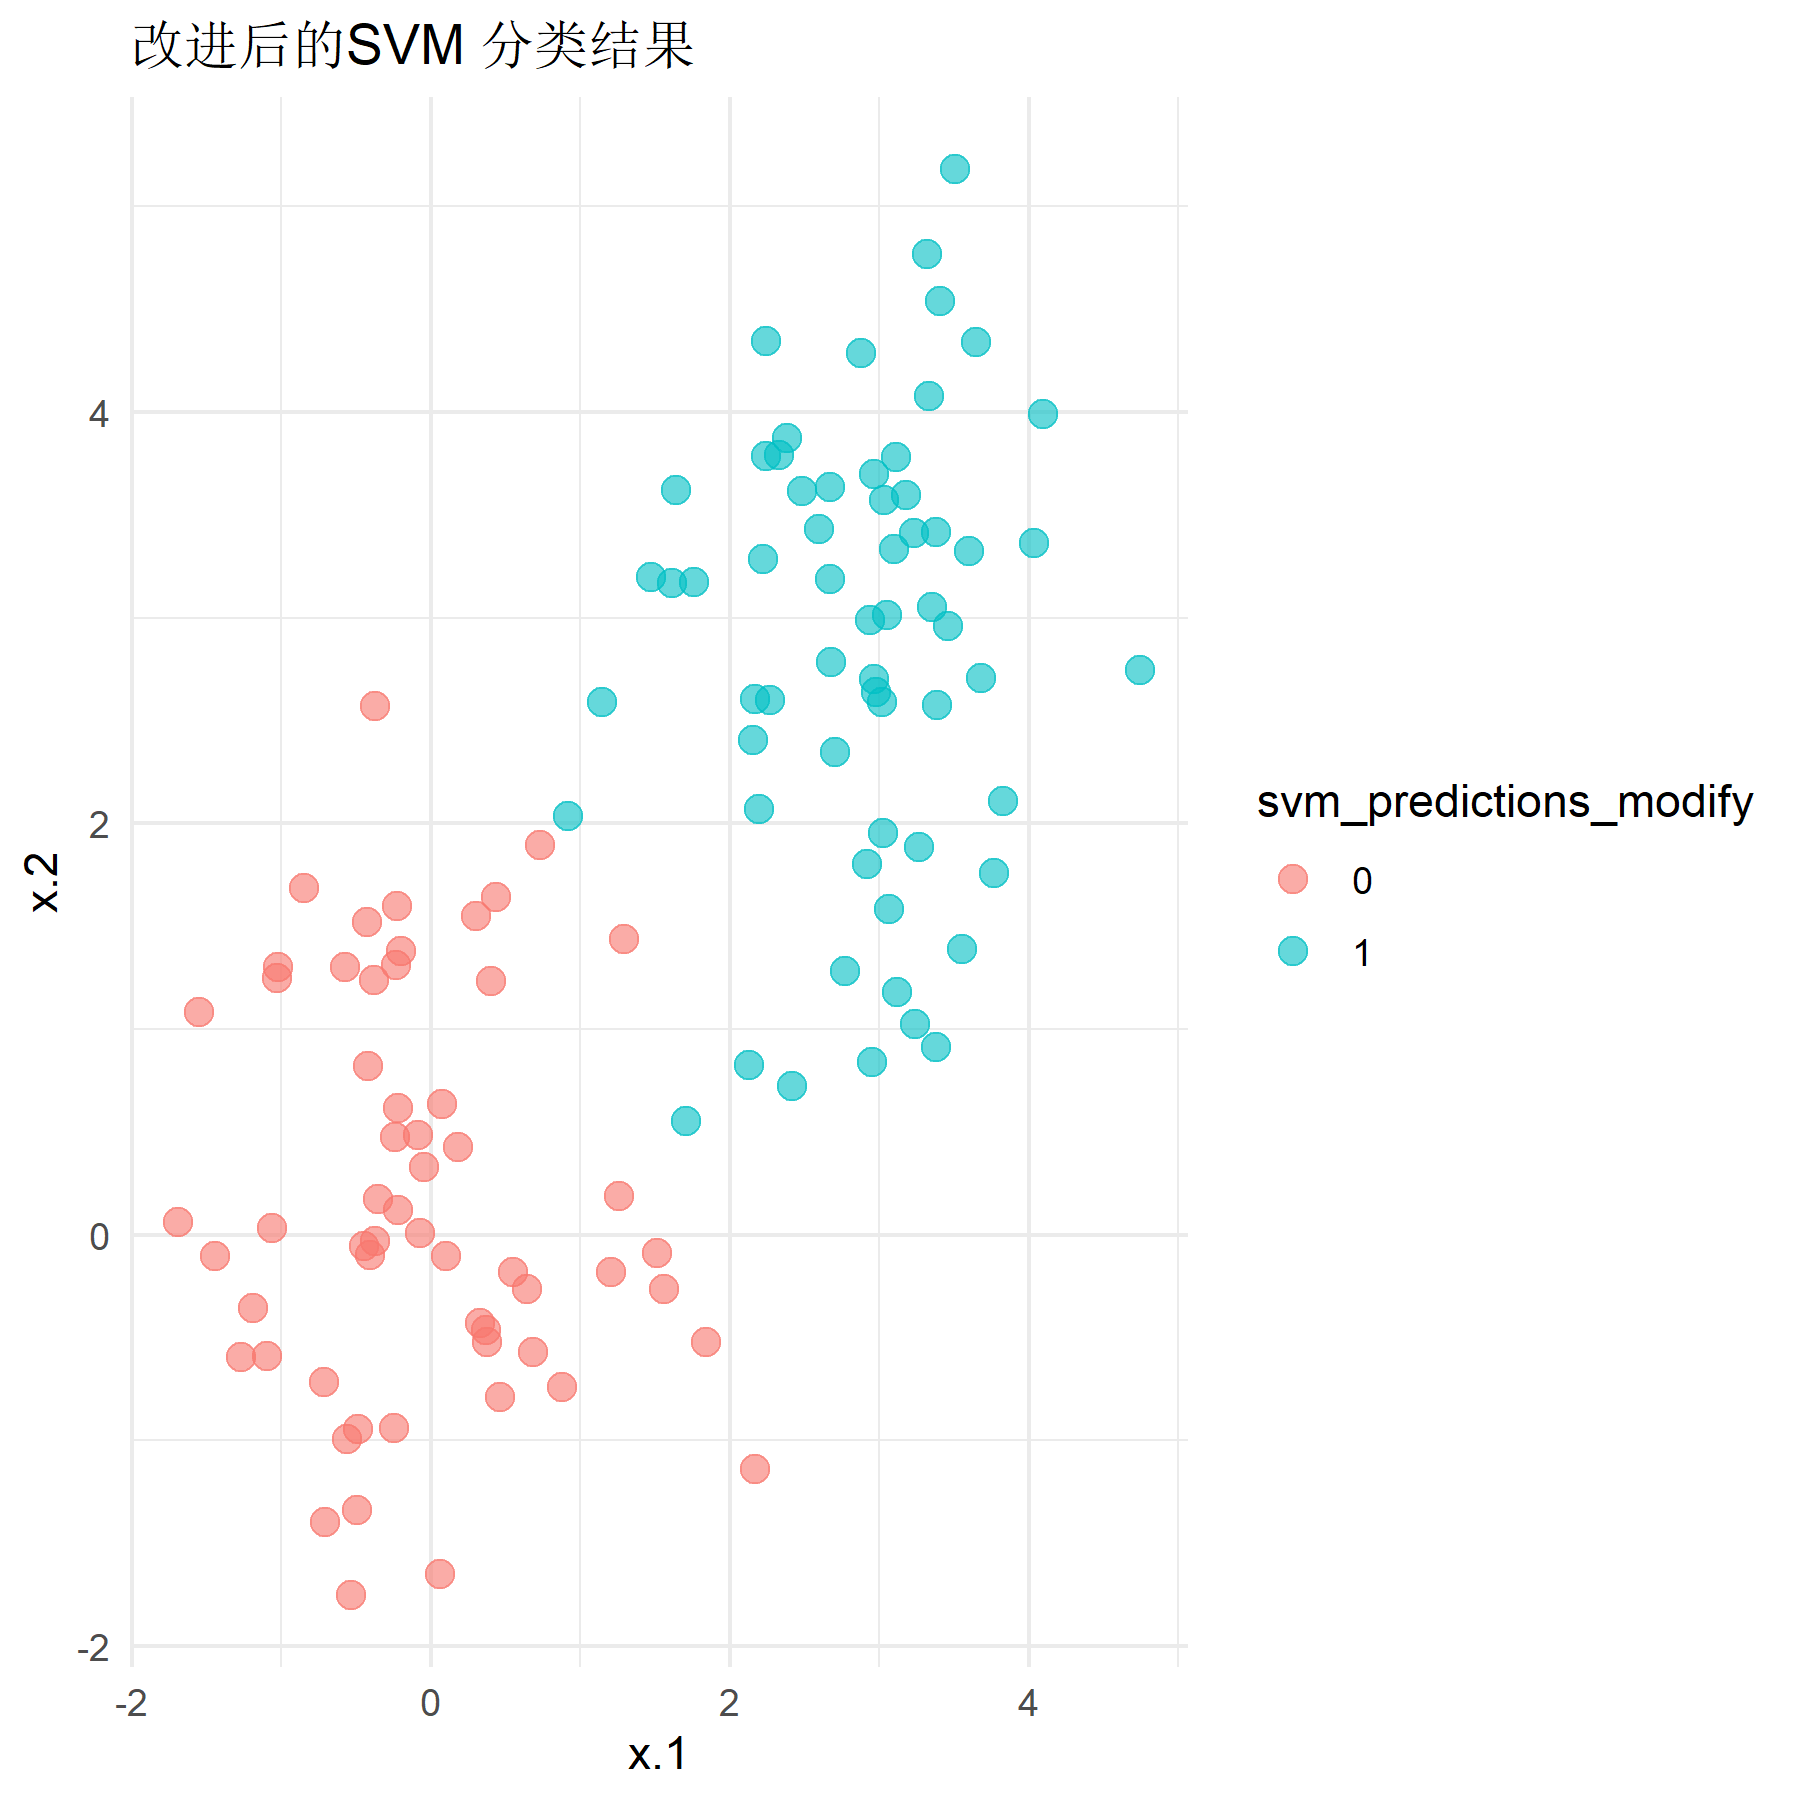
\includegraphics[width=0.4\textwidth]{12.png}
	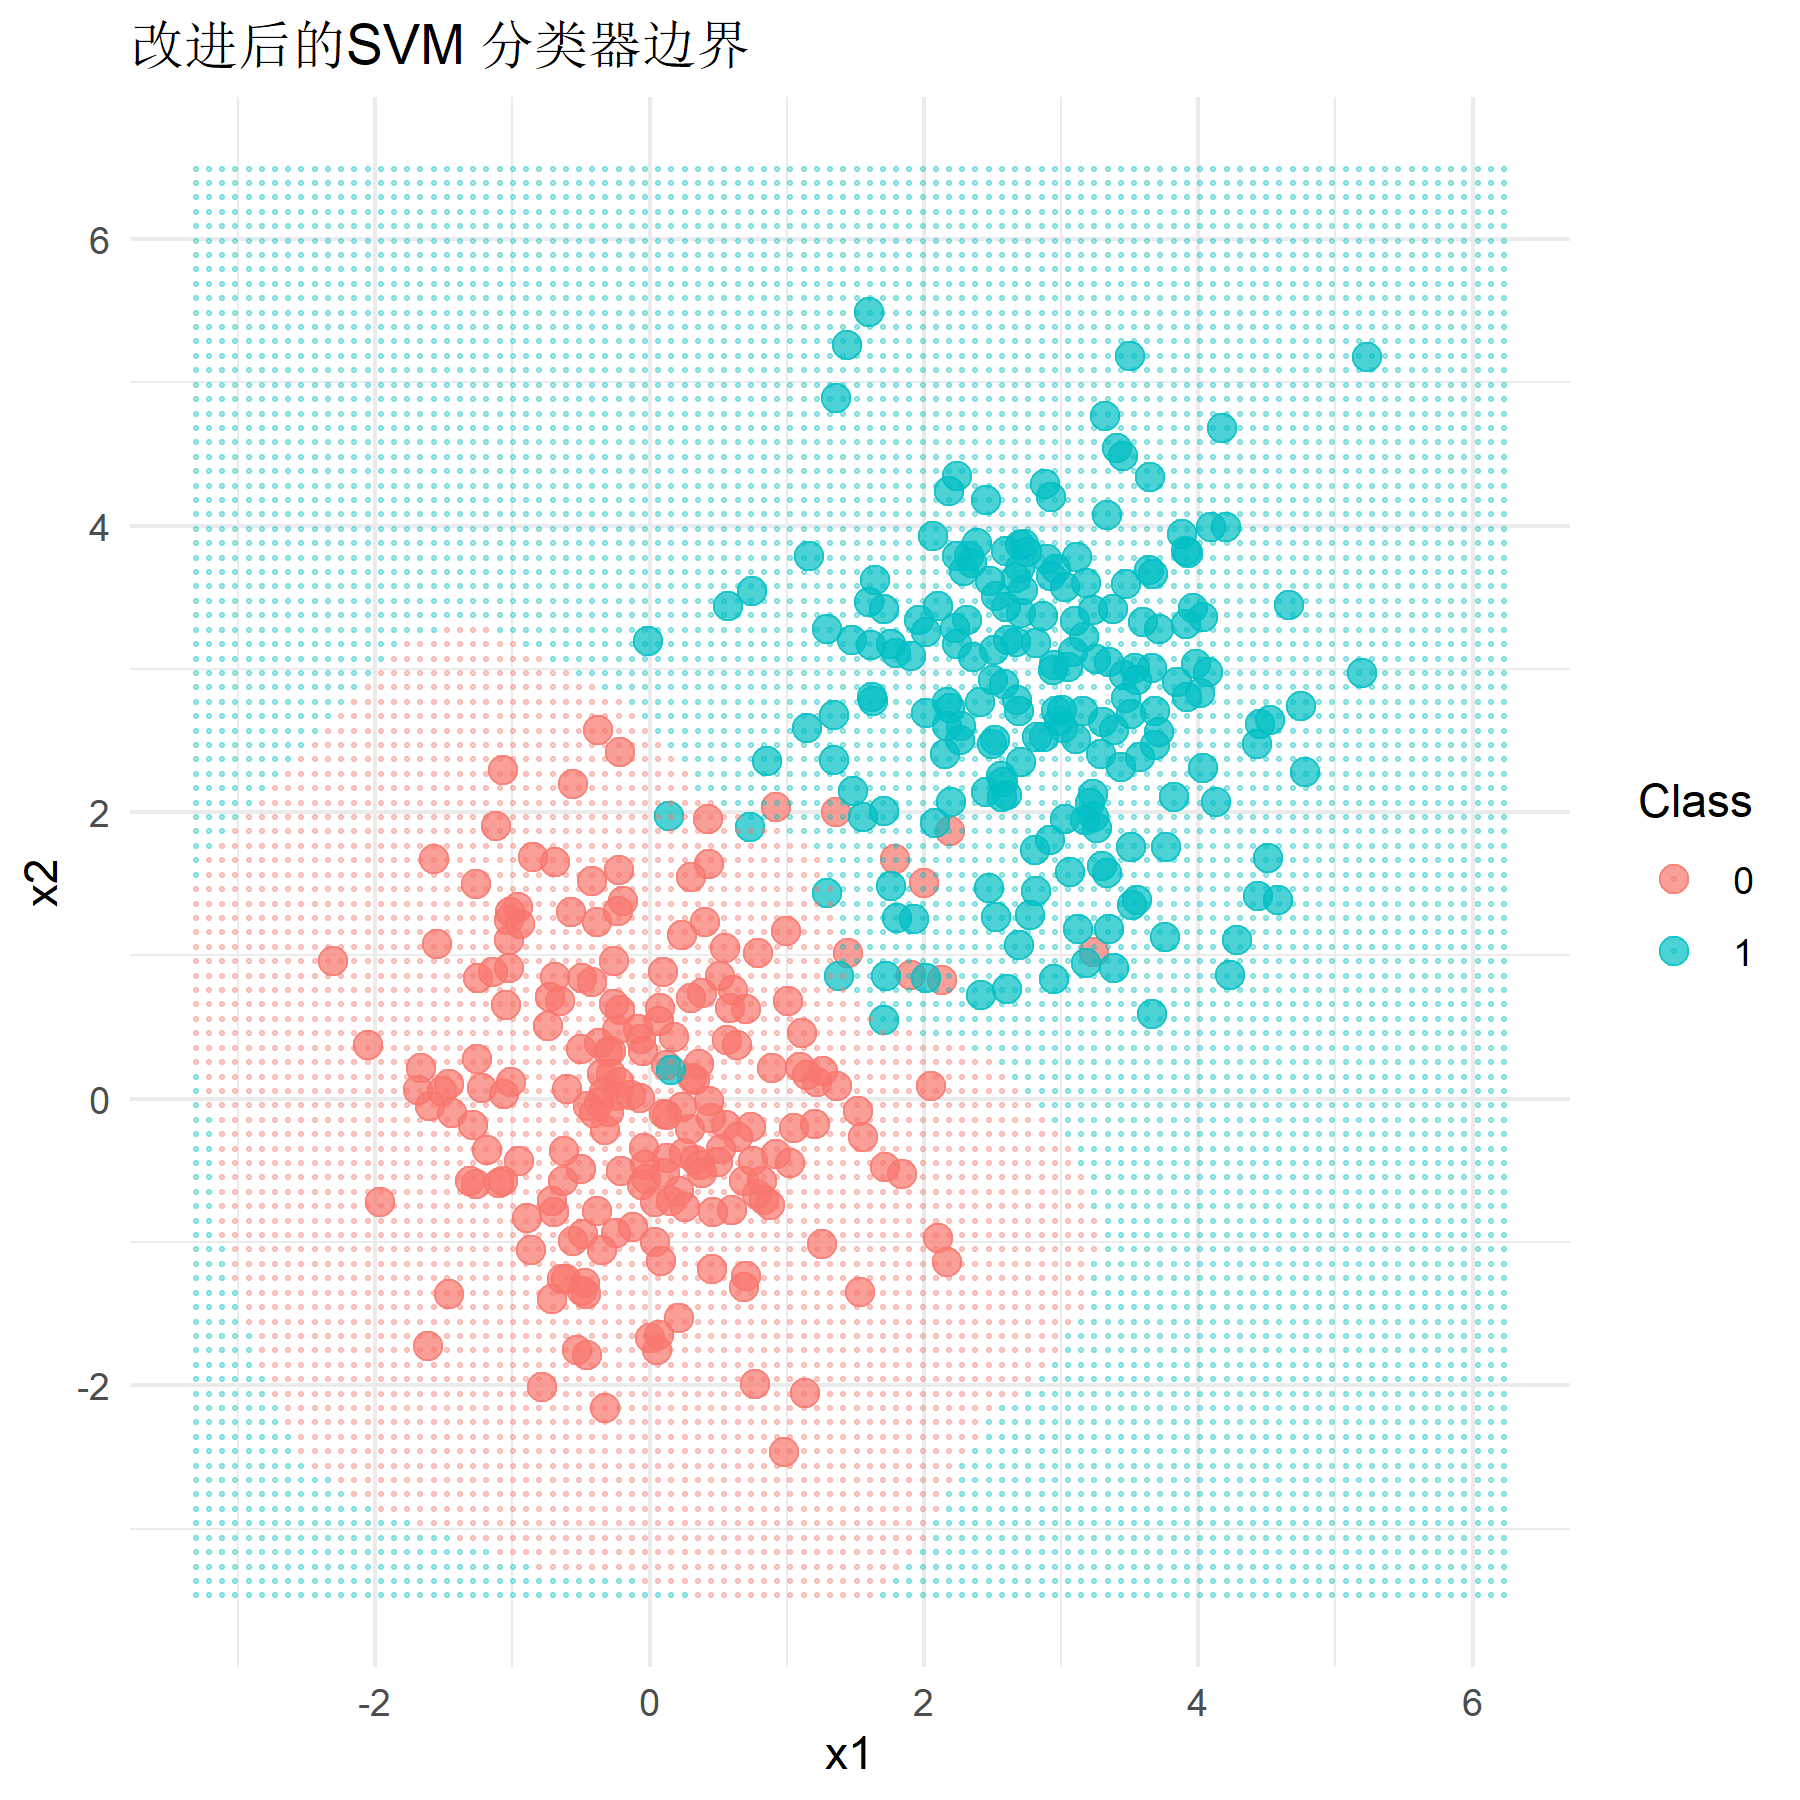
\includegraphics[width=0.4\textwidth]{13.png}
\end{figure}

\section{文献调研}	

硬间距SVM要求构建的分类超平面完全正确的分类所有训练数据,但由于实际样本被假设成线性可分的条件太强,为避免过拟合,更多时候需要考虑软间距(soft-margin)SVM模型。

所谓软间距,就是允许一些点不满足线性可分的约束条件,即:$y_i\left(w^Tx_i+b\right)<1$。当然,为保证拟合模型仍然为一种SVM方法的“本性”,我们希望这样的点不能太多,因此要对违反约束的样本点$(x_i, y_i)$施加一定的非负惩罚(松弛变量)$\delta_i$:

\begin{equation}
	\delta_i=max\{0, 1-y_i\left(w^Tx_i+b\right)\}=
	\begin{cases}
		0, y_i\left(w^Tx_i+b\right)\geq1\         \\                                           
		1-y_i\left(w^Tx_i+b\right),\ y_i\left(w^Tx_i+b\right)<1
	\end{cases}                               
\end{equation}

这样就可以得到软间隔SVM的基本数学模型:

\begin{equation}
	\begin{cases}
		\mathop{min}\limits_{w,\ b,\ \delta_i} {{\frac{1}{2}||w||}^2+c\sum_{i=1}^{n}\delta_i}         \\                                           
		st:\ y_i(w^Tx_i+b)+\delta_i\geq1,\ \delta_i\geq0,\ i=1,\cdots,n
	\end{cases}                               
\end{equation}

值得注意的是,每一个样本都有一个对应的松弛变量,表征该样本不满足约束的程度;$c>0$为惩罚参数,其值越大,对分类的惩罚越大。跟硬间隔SVM一样,先用拉格朗日乘子法得到拉格朗日函数,再求其对偶问题。

在正则化的框架下,软间隔SVM的基本数学模型结构还可改写为:

\begin{equation}
	\mathop{min}\limits_{w,\ b,\ \delta_i} {{\frac{1}{2}||w||}^2+c\sum_{i=1}^{n}\delta_i}                          
\end{equation}

其中学习机、损失项、正则化项分别定义为:

\begin{itemize}
	\setlength{\parsep}{0ex} %段落间距
	\setlength{\topsep}{2ex} %列表到上下文的垂直距离
	\setlength{\itemsep}{1ex} %条目间距
	\item \textbf{学习机}:$f\left(w\right)=w^Tx+b$;		
	\item \textbf{损失项}:$c\sum_{i=1}^{n}\delta_i$;
	\item \textbf{正则项}:$\frac{1}{2}w^Tw={\frac{1}{2}||w||}^2$。
\end{itemize}

基于软间隔SVM模型,理论上的拓展主要集中在模型\textbf{损失项与正则项}两个方面,针对这两个方面,接下来将分别选取一篇文献,对其改进模型、求解算法与创新点进行简单的书面总结。

\subsection{正则项拓展:柔性套索惩罚\upcite{2}}
\subsubsection{模型重述}

柔性套索(Pliable lasso)是一种新的互动模型,由Robert Tibshirani和Jerome Friedman于2018年提出。该模型是原始套索问题的扩展,允许套索回归模型接受修改变量、预测因子和结果。原始的套索(Lasso)问题本质上是将1-范数作为正则项,而柔性套索是在此基础上的改进。1-范数支持向量机的缺点之一是,在一些输入高度相关的情况下,并且所有输入都与输出相关,1-范数惩罚最终会挑选出少数输入,并将其余的减少到零,这意味着“群体选择”将是对1范数支持向量机的挑战。

柔性套索惩罚允许估计协变量X的主要影响以及协变量与一组修饰符Z之间的相互作用影响,以处理相互作用效应。为了处理变量选择并帮助选择相关变量组,引入修正变量$Z$,并将柔性套索作为正则项(惩罚项),得到具有柔性套索惩罚的SVM目标函数:

\begin{equation}
	\min_{\beta, h} \left( \frac{1}{n} \sum_{i=1}^n (1 - y_i (\beta_0 + x_i^T \beta))_+^2 + \lambda_1 \left( \sum_{j=1}^p \|\beta_j\|_1 + \sum_{j=1}^p \|h_j\|_1 \right) + \frac{\lambda_2}{2} \left( \|\beta\|_2^2 + \sum_{j=1}^p \|h_j\|_2^2 \right) \right)
\end{equation}

其中,学习机、损失项和正则化项(惩罚项)定义如下:

\begin{itemize}
	\setlength{\parsep}{0ex} %段落间距
	\setlength{\topsep}{2ex} %列表到上下文的垂直距离
	\setlength{\itemsep}{1ex} %条目间距
	\item \textbf{学习机}:$y = \beta_0 + Z h_0 + \sum_{j=1}^p X_j (\beta_j + Z h_j) + \epsilon_i$;		
	\item \textbf{损失项}:损失平方和(hinge函数)$\frac{1}{n} \sum_{i=1}^n (1 - y_i (\beta_0 + x_i^T \beta))^2$;
	\item \textbf{正则项}:柔性套索惩罚 $\lambda_1 \left( \sum_{j=1}^p \|\beta_j\|_1 + \sum_{j=1}^p \|h_j\|_1 \right) + \frac{\lambda_2}{2} \left( \|\beta\|_2^2 + \sum_{j=1}^p \|h_j\|_2^2 \right)$。
\end{itemize}

\subsubsection{求解算法与创新点}

在目标函数优化的求解过程中,主要使用\textbf{块方向坐标下降过程}(the block-wise coordinate descent procedure)优化目标函数:

\begin{algorithm}
	\caption{SVM pliable lasso模型的算法(Plasso-SVM)}
	\begin{algorithmic}[1]
		\STATE \textbf{初始化:}
		\FOR{每个 \(\lambda\) 递减}
		\STATE 初始化:设置所有 \((\hat{\beta}_0, \hat{\beta}_j) = 0\),\((\hat{\theta}_0, \hat{\theta}_j) = 0\) (\(j = 1, 2, \ldots, p\))
		\STATE 计算 \(\tilde{n}\),\(b = 1(y_i(\tilde{n}) < 1)\) 和 \(r = [1 - y(\tilde{n})]_+\)
		\STATE 计算 \(\hat{\beta}_0\) 和 \(\hat{\theta}_0\)
		\FOR{每个 \(j \in \{1, 2, \ldots, p\}\)}
		\IF{\((\hat{\beta}_j, \hat{\theta}_j) = 0\)}
		\STATE 跳到下一个 \(j\)
		\ELSE
		\STATE 计算 \(\hat{\beta}_j\),然后检查 \(\hat{\theta}_j = 0\)
		\ENDIF
		\IF{\(\hat{\theta}_j = 0\)}
		\STATE 使用计算出的 \(\hat{\beta}_j\) 更新 \(\beta_j\),然后跳到下一个 \(j\)
		\ELSE
		\STATE 使用广义梯度下降法计算 \((\hat{\beta}_j, \hat{\theta}_j)\)
		\ENDIF
		\ENDFOR
		\ENDFOR
	\end{algorithmic}
\end{algorithm}

本篇文章在过去已有模型的基础上再次进行了改进,创造性地把柔性套索(优化后的1-范数)作为惩罚项(正则项)引入软间隔SVM模型中,\textbf{创新点}有如下几条:

\begin{itemize}
	\setlength{\parsep}{0ex} %段落间距
	\setlength{\topsep}{2ex} %列表到上下文的垂直距离
	\setlength{\itemsep}{1ex} %条目间距
	\item \textbf{可调套索惩罚的应用}:将可调套索惩罚应用于支持向量机,能够有效估计协变量与修饰变量之间的交互作用。
	\item \textbf{交互项排除机制}:通过可调套索,能够在相应主效应为零时自动排除交互项,提高模型的解释性和简洁性。
	\item \textbf{平方铰链损失结合块坐标下降算法}:使用该组合优化目标函数,在模拟和实际数据(结肠癌和前列腺癌数据集)上验证了方法的有效性。
\end{itemize}

\subsection{损失项拓展:快速截断Huber损失\upcite{3}}
\subsubsection{模型重述}

支持向量机作为一种有用的分类工具,在许多领域得到了广泛的应用。然而,在非常大的样本数据集上,它可能会导致计算上的不可行性。为了解决这一问题,该文章提出了一种新颖的\textbf{带有截断Huber损失的稀疏鲁棒支持向量机模型},即$L_{th}$-SVM,其基本数学模型如下:

\begin{equation}
	\min_{w \in \mathbb{R}^n, b \in \mathbb{R}} \frac{1}{2} \|w\|^2 + \gamma \sum_{i=1}^m \ell_{th}(1 - y_i(\langle w, x_i \rangle + b)) 
\end{equation}

也可写作:

\begin{equation}
	\min_{w \in \mathbb{R}^n, b \in \mathbb{R}} \frac{1}{2} \|w\|^2 + \gamma \sum_{i=1}^m \ell_{th}(h) 
\end{equation}

其中,学习机、损失项和正则化项(惩罚项)定义如下:

\begin{itemize}
	\setlength{\parsep}{0ex} %段落间距
	\setlength{\topsep}{2ex} %列表到上下文的垂直距离
	\setlength{\itemsep}{1ex} %条目间距
	\item \textbf{学习机}:$h:= \mathbf{1} - \mathcal{G}\mathbf{w} - b\mathbf{y} \in \mathbb{R}^{m} $,其中$\begin{aligned}  
				\mathcal{G} &:= \left[ \begin{array}{cccc}  
					y_{1}x_{1} & y_{2}x_{2} & \cdots & y_{m}x_{m}  
				\end{array} \right]^{\top} \in \mathbb{R}^{m \times n}
		\end{aligned}  $;		
	\item \textbf{损失项}:快速截断Huber损失(Truncated Huber Loss):
	
	$\ell_{\text{th}}(t) = \begin{cases}   
		1, & \text{if } t > 1 + \frac{\delta}{2}, \\  
		t - \frac{\delta}{2}, & \text{if } t \in \left[\delta, 1 + \frac{\delta}{2}\right], \\  
		\frac{t^2}{2\delta}, & \text{if } t \in [0, \delta), \\  
		0, & \text{if } t < 0.   
	\end{cases}$;
	
	\item \textbf{正则项}:L2正则化 $\frac{1}{2}w^Tw={\frac{1}{2}||w||}^2$。
\end{itemize}

\subsubsection{求解算法与创新点}

针对$L_{th}$-SVM问题,文章提出了一种新颖高效的乘子与工作集交替方向的方法($L_{th}$-ADMM),证明了$L_{th}$-ADMM产生的序列是$L_{th}$-SVM的局部最小值,并且在工作集很小的情况下具有较低的计算复杂度。大量的数值实验表明,$L_{th}$-ADMM能够提供更高的预测精度,提供更少的支持向量,并且运行速度快,特别是在大规模数据集设置中。其求解算法大致如下:  
	
\begin{breakablealgorithm} 
	\caption{$L_{th}$-ADMM算法求解截断Huber损失SVM}  
	\begin{algorithmic}[1]  
		\REQUIRE  
		训练数据:$\{(x_i, y_i)\}_{i=1}^m$,其中 $x_i \in \mathbb{R}^n$,$y_i \in \{-1, 1\}$  
		参数:$\gamma, \nu, \delta, K$(最大迭代次数)  
		\ENSURE 
		近似最优解 $(w^k, b^k)$  
		
		\STATE \textbf{初始化:}  
		$(w^0, b^0, h^0, \alpha^0) = 0$  // 初始化为适当大小的零向量/标量  
		$\mu = 1.618$  // 对偶步长(迭代过程中固定)  
		
		\FOR{$k = 0$ \TO $K-1$}  
		\STATE // 步骤1:计算工作集 $J_k$  
		\IF{$\delta + \kappa\gamma \in (0, 2)$}  
		\STATE 根据 $s_k$ 和 $\alpha^k$ 计算 $\Gamma_{1k}$,$\Gamma_{2k}$  
		\STATE $J_k = \Gamma_{1k} \cup \Gamma_{2k}$  
		\ELSE  
		\STATE 根据 $s_k$ 和 $\alpha^k$ 计算 $I_k$  
		\STATE $J_k = I_k$  
		\ENDIF  
		
		\STATE // 步骤2:更新 $h^{k+1}$  
		\STATE $s_k = h^k - \alpha^k / \nu$  
		\FOR{$i \in J_k$}  
		\IF{$i \in \Gamma_k$}  
		\STATE $h^{k+1}_i = \text{prox}_{\gamma/\nu L_{th}}(s_k)_i$  
		\ELSE  
		\STATE $h^{k+1}_i = s_{k_i}$  
		\ENDIF  
		\ENDFOR  
		
		\STATE // 步骤3:更新 $w^{k+1}$  
		\STATE $\varphi_k = -(h^{k+1} + b^k y - 1 + \alpha^k / \nu)$  
		\IF{$n \leq |J_k|$}  
		\STATE $w^{k+1} = (I + \nu G_{J_k}^\top G_{J_k})^{-1} \nu G_{J_k}^\top \varphi_k^{J_k}$  
		\ELSE  
		\STATE $w^{k+1} = \nu G_{J_k}^\top (I + \nu G_{J_k} G_{J_k}^\top)^{-1} \varphi_k^{J_k}$  
		\ENDIF  
		
		\STATE // 步骤4:更新 $b^{k+1}$  
		\STATE $\chi^k = -G w^{k+1} + 1 - h^{k+1} - \alpha^k / \nu$  
		\STATE $b^{k+1} = \langle y, \chi^k \rangle / m$  
		
		\STATE // 步骤5:更新 $\alpha^{k+1}$  
		\STATE $\zeta^{k+1} = h^{k+1} - 1 + G w^{k+1} + b^{k+1} y$  
		\FOR{$i \in J_k$}  
		\STATE $\alpha^{k+1}_i = \alpha^k_i + \mu\nu\zeta^{k+1}_i$  
		\ENDFOR  
		\FOR{$i \in J_k^c$}  
		\STATE $\alpha^{k+1}_i = 0$  
		\ENDFOR  
		
		\STATE // 检查停止准则(可选)  
		\IF{满足停止准则}  
		\STATE \textbf{break}  
		\ENDIF  
		\ENDFOR  
	\end{algorithmic}  
\end{breakablealgorithm} 

本文的创新点主要包括以下几个方面:

\begin{itemize}
	\setlength{\parsep}{0ex} %段落间距
	\setlength{\topsep}{2ex} %列表到上下文的垂直距离
	\setlength{\itemsep}{1ex} %条目间距
	\item \textbf{截断Huber损失函数的提出}:提出了一种新的截断Huber损失函数,该函数能够在保持稀疏性的同时,增加对异常值的鲁棒性。与现有的hinge损失、huberized pinball损失和Huber损失相比,截断Huber损失函数在稀疏性和鲁棒性方面表现出更优的性能。
	\item \textbf{稀疏鲁棒SVM模型的构建}:基于截断Huber损失函数,构建了新的稀疏鲁棒支持向量机模型(Lth-SVM)。该模型不仅继承了SVM分类能力强、理论框架完善等优点,还通过引入截断Huber损失函数提高了模型的稀疏性和鲁棒性,使其在处理大规模分类问题时更加有效。
	\item \textbf{一阶最优性条件的建立}:为$L_{th}$-SVM模型建立了基于新引入的P-稳定点的一阶必要和充分条件,定义了$L_{th}$支持向量和工作集。这些条件为算法设计提供了理论基础,同时也证明了所有$L_{th}$支持向量仅占整个训练集的一小部分,这为后续开发高效算法提供了可能。
	\item \textbf{$L_{th}$-ADMM求解算法的设计}:提出了一种具有工作集的新型交替方向乘子法($L_{th}$-ADMM)来求解$L_{th}$-SVM。该算法通过引入工作集策略,显著降低了每次迭代中的计算复杂度,使得算法在处理大规模数据集时能够快速收敛。同时,理论证明表明,该算法生成的序列能够收敛到$L_{th}$-SVM的一个局部极小值。
\end{itemize}

\begin{thebibliography}{99}
	\bibitem{1} Cortes C, Vapnik V. Support-vector networks[J]. Machine learning, 1995, 20(3): 273-297.
	\bibitem{2} Asenso, T. Q., Wang, P., \& Zhang, H. (2022). Pliable lasso for the support vector machine. Communications in Statistics - Simulation and Computation, 53(2), 786–798.
	\bibitem{3} Huajun Wang, Yuanhai Shao, Fast truncated Huber loss SVM for large scale classification,	Knowledge-Based Systems, Volume 260, 2023.
\end{thebibliography}

\end{document} 
